%%%%%%%%%%%%%%%%%%%% book.tex %%%%%%%%%%%%%%%%%%%%%%%%%%%%%
%
% sample root file for the chapters of your "monograph"
%
% Use this file as a template for your own input.
%
%%%%%%%%%%%%%%%% Springer-Verlag %%%%%%%%%%%%%%%%%%%%%%%%%%


% RECOMMENDED %%%%%%%%%%%%%%%%%%%%%%%%%%%%%%%%%%%%%%%%%%%%%%%%%%%
\documentclass[pdftex,12pt, oneside]{book}

% choose options for [] as required from the list
% in the Reference Guide, Sect. 2.2
\usepackage[paperwidth=8.5in, paperheight=13in]{geometry}

\usepackage{makeidx}         % allows index generation
\usepackage{graphicx}        % standard LaTeX graphics tool
                             % when including figure files
%\usepackage{multicol}        % used for the two-column index
\usepackage[bottom]{footmisc}% places footnotes at page bottom
\usepackage[english]{babel}
\usepackage{enumerate}
\usepackage{paralist}
\usepackage{float}
\usepackage{gensymb}  
\usepackage{listings}
%\usepackage{siunitx}
% etc.
% see the list of further useful packages
% in the Reference Guide, Sects. 2.3, 3.1-3.3

\newcommand{\HRule}{\rule{\linewidth}{0.5mm}}

\makeindex             % used for the subject index
                       % please use the style svind.ist with
                       % your makeindex program


%%%%%%%%%%%%%%%%%%%%%%%%%%%%%%%%%%%%%%%%%%%%%%%%%%%%%%%%%%%%%%%%%%%%%

\begin{document}

%\author{Priyanto Tamami}
%\title{BUKU PETUNJUK OPERASIONAL SISTEM INFORMASI GEOGRAFIS UNTUK PBB-P2 DENGAN MAPINFO VERSI 8.0}
%\date{22 Desember 2015}
%\maketitle

\begin{titlepage}

\begin{center}
{\large BUKU PETUNJUK OPERASIONAL SISTEM INFORMASI GEOGRAFIS UNTUK PBB-P2 DENGAN MAPINFO VERSI 8.0}

\HRule\\[1cm]

PERIODE PENILAIAN TAHUN 2016\\[1cm]


\includegraphics[width=0.5\textwidth]{./resources/logo}\\[1cm]

Oleh :\\
Priyanto Tamami, S.Kom.\\
NIP 19840409 201001 1 025\\
Dinas Pendapatan dan Pengelolaan Keuangan\\
Pemerintah Kabupaten Brebes\\[1cm]

\vfill

Tim Penilai\\
Jabatan Fungsional Pranata Komputer\\
Badan Pusat Statistik\\
Brebes, 22 Desember 2015
\end{center}

\end{titlepage}

\frontmatter%%%%%%%%%%%%%%%%%%%%%%%%%%%%%%%%%%%%%%%%%%%%%%%%%%%%%%

%\include{dedic}
%\include{pref}

\begin{center}
{\huge \bfseries Lembar Pengesahan}\\[0.4cm]

\begin{tabular}{l c p{10cm}}
  Nama Kegiatan & : & Membuat Petunjuk Operasional Sistem Komputer \\
  Judul & : & BUKU PETUNJUK OPERASIONAL SISTEM INFORMASI GEOGRAFIS UNTUK PBB-P2 DENGAN MAPINFO VERSI 8.0 \\
\end{tabular}\\[2cm]

\begin{tabular}{c c}
  Disetujui oleh : & Disusun Oleh \\
  Kepala Seksi Pendataan, Penetapan, dan Keberatan & Pranata Komputer \\
  Pada tanggal 22 Desember 2015 & Selesai tanggal : 21 Desember 2015 \\
  & \\
  & \\
  & \\
  Fetiana Dwiningrum, SIP, M.Si. & Priyanto Tamami, S.Kom \\
  NIP 19880223 200701 2 001 & NIP 19840409 201001 1 025
\end{tabular}

\end{center} 

\tableofcontents
\listoffigures

\mainmatter%%%%%%%%%%%%%%%%%%%%%%%%%%%%%%%%%%%%%%%%%%%%%%%%%%%%%%%
%\include{part}
%\include{chapter}
%\include{chapter}
%\appendix
%\include{appendix}

\chapter{KONSEP SISTEM INFORMASI GEOGRAFIS (SIG)}

\begin{enumerate}[A.]
\item{Definisi}

Sistem Informasi Geografis merupakan gabungan dari tiga unsur pokok yaitu: \textbf{sistem}, \textbf{informasi}, dan \textbf{geografis}. Istilah \textbf{sistem} sangat populer digunakan untuk mendeskripsikan banyak hal, khususnya untuk aktifitas-aktifitas yang diperlukan dalam pemrosesan data.

\textbf{Sistem} dapat didefinisikan sebagai sekumpulan objek, ide yang disertai dengan keterhubungannya dalam mencapai tujuan atau sasaran bersama. Atau sistem dapat juga dikatakan sebagai keterkaitan dan keterpaduan kerja antar komponen dengan berbagai fungsi untuk mendapatkan suatu hasil.

\textbf{Informasi} adalah data yang berformat dan terorganisasi dengan baik agar mudah dikelola untuk dianalisis atau diproses.

\textbf{Sistem Informasi} adalah suatu jaringan kegiatan mulai dari pengumpulan data, manipulasi, pengelolaan dan analisis serta menjabarkannya menjadi informasi.

Dari pengertian di atas dapat disimpulkan berbagai definisi Sistem Informasi Geografis diantaranya yaitu :

\begin{itemize}

\item \textbf{Sistem Informasi Geografis} adalah sistem informasi yang direkayasa untuk bekerja dengan data yang berreferensi keruangan (geografis)

\item \textbf{Sistem Informasi Geografis} adalah satuan tata cara yang digunakan untuk menyimpan, memanipulasi dan menganalisis data dengan berreferensi geografis baik manual maupun digital.

\item \textbf{Sistem Informasi Geografis} adalah sistem yang berisi data berreferensi geografis yang dapat dianalisis dan dikonversi menjadi informasi untuk suatu tujuan tertentu atau pemanfaatan tertentu. Hal utama pada SIG adalah analisis data untuk mendapatkan informasi baru.

\item \textbf{Sistem Informasi Geografis} adalah suatu sistem komputer yang digunakan untuk memasukkan, menyimpan, memeriksa, mengintegrasikan, memanipulasi, menganalisis, dan menampilkan data yang berhubungan dengan posisi-posisi di permukaan bumi.

\item \textbf{Sistem Informasi Geografis} adalah sistem yang berbasis komputer yang digunakan untuk menyimpan dan memanipulasi informasi-informasi geografis. SIG dirancang untuk mengumpulkan, menyimpan, dan menganalisis objek-objek dan fenomena dimana lokasi geografis merupakan karaketeristik yang penting atau kritis untuk dianalisis. Dengan demikian, SIG merupakan sistem komputer yang memiliki empat kemampuan berikut dalam menangani data yang berreferensi geografis: 
\begin{inparaenum}[(a)]
\item masukan/input, 
\item manajemen data (penyimpanan dan pemanggilan data), 
\item analisis dan manipulasi data, 
\item keluaran / output.
\end{inparaenum}

\end{itemize}

\item{Komponen SIG}

SIG merupakan suatu sistem yang kompleks yang biasanya terintegrasi dengan sistem komputer. Komponen SIG terdiri dari :

\begin{itemize}
\item Perangkat Keras (\textit{Hardware})

Perkembangan dunia komputer saat ini begitu pesat dengan spesifikasi yang tinggi seperti kemampuan prosesor yang semakin cepat, kapasitas \textit{harddisk} dan memori (RAM) yang semakin besar, sudah sangat memenuhi persyaratan pengolahan data yang dibutuhkan bagi suatu pekerjaan SIG.

Perangkat keras yang lazim digunakan berupa, PC, \textit{mouse}, \textit{digitizer}, \textit{printer}, \textit{scanner}, dan \textit{plotter}.

\item Perangkat Lunas (\textit{Software})

Untuk melakukan suatu pekerjaan SIG berbasis komputer sangat dibutuhkan perangkat lunak pengolahnya. Sekarang tersedia berbagai perangkat lunak yang beredar di pasar dan mudah didapat. Diantaranya yang lazim digunakan adalah : AutoCAD, MapInfo, R2V, ArcGIS, ArcView, dll. Namun yang akan kita gunakan saat ini adalah MapInfo, karena \textit{software} inilah yang digunakan Direktorat Jenderal Pajak untuk mengelola data spasial Pajak Bumi dan Bangunan Perdesaan dan Perkotaan sehingga dalam implementasinya tidak menimbulkan permasalahan baru mengenai konversi data, atau perbedaan perangkat simpanan data yang digunakan.

\item Data dan Informasi Geografi

Data dan informasi geografi dapat diperoleh dengan mendijitasi data spasialnya secara langsung dari peta dan memasukkan data atribut pada data spasial itu. SIG juga memberikan kemudahan untuk mengumpulkan dan menyimpan suatu data dan informasi geografis yang telah dibuat dari perangkat lunak lainnya dengan cara meng\textit{import} kedalam perangkat lunak yang dipakai.

\item Manajemen

Suatu pekerjaan SIG akan berhasil dengan baik jika dikerjakan dengan manajemen yang baik.

\end{itemize}

\item{Data dan Informasi}

Pembahasan mengenai sistem informasi diawali dengan pendefinisian secara fungsional tentang data dan informasi. Istilah data dan informasi sering digunakan secara bergantian dan saling tertukar namun melalui kesepakatan umum dapat diartikan sebagai simbol-simbol pengganti yang menggambarkan peristiwa, aktifitas, konsep, dan objek-objek penting.

Macam data pada pekerjaan SIG yaitu :

\begin{enumerate}[\itshape 1.]

  \item \textit{Data Grafis}
    
    \begin{itemize}
    
      \item Berwujud Titik (non dimensional)

    Contoh : objek ibukota (kecamatan, kabupaten, dst), gunung, bukit, letak suatu objek (rumah sakit, pos polisi, restoran, dsb).

      \item Berwujud Garis / line (satu dimensi)

    Contoh : Objek jalan, rel kereta api, sungai kecil, kontur, dsb.

      \item Berwujud Area / polygon (dua dimensi)

    Contoh: Batas administrasi penggunaan lahan, blok permukiman, sungai besar, dsb.

    \end{itemize}

  \item \textit{Data Atribut}

  Data atribut adalah data atau informasi yang menjelaskan perihal tentang data grafis.
  
  Contoh : nama ibukota, nama dan tinggi gunung, nama jalan, nama sungai, nama kecamatan, jenis penggunaan lahan.
  
\end{enumerate}  

\item Aplikasi SIG

Penerapan SIG dapat digunakan pada banyak bidang, misalnya :

  \begin{enumerate}[(a)]
  
    \item Sumber Daya Alam

    Inventarisasi SDA, Pengelolaan SDA, Kesesuaian Lahan untuk pertanian, perkebunan, kehutanan.

    \item Perencanaan

    Perencanaan Tata Ruang Wilayah/Kota. Perencanaan Lokasi Permukiman, Relokasi Permukiman dan Industri

    \item Lingkungan

    Manajemen Rawan Bencana, Pemetaan Pencemaran (Sungai, Danau, Laut)

    \item Utility

    Manajemen Informasi Jaringan Pipa Air Minum, Fasilitas Umum lainnya.

    \item Ekonomi, Bisnis, dan Marketing
  
    Penentuan Lokasi Pasar Swalayan, Bank, Kantor Cabang.

    \item Telekomunikasi

    Sistem Informasi Pelanggan, Jaringan Telekomunikasi, Fasilitas Umum Telekomunikasi.

    \item Kelautan

    Pemetaan SDA Laut, Manajemen SDA Laut, Daerah Penangkapan Ikan, Kesesuaian Lahan Tambak.

    \item Transportasi

    Jaringan Transportasi, Penentuan Rute ALternatif Transportasi
    
  \end{enumerate}

\end{enumerate}
\chapter{PENGENALAN SOFTWARE}

\begin{enumerate}[\bfseries A.]

  \item \textbf{Membuka Program}
  
  \begin{enumerate}[1.]
  
    \item Pilih Start -\textgreater Program -\textgreater MapInfo -\textgreater MapInfo 8. Muncul tampilan jendela berikut :
    
    \begin{figure}[H]
      \centering
      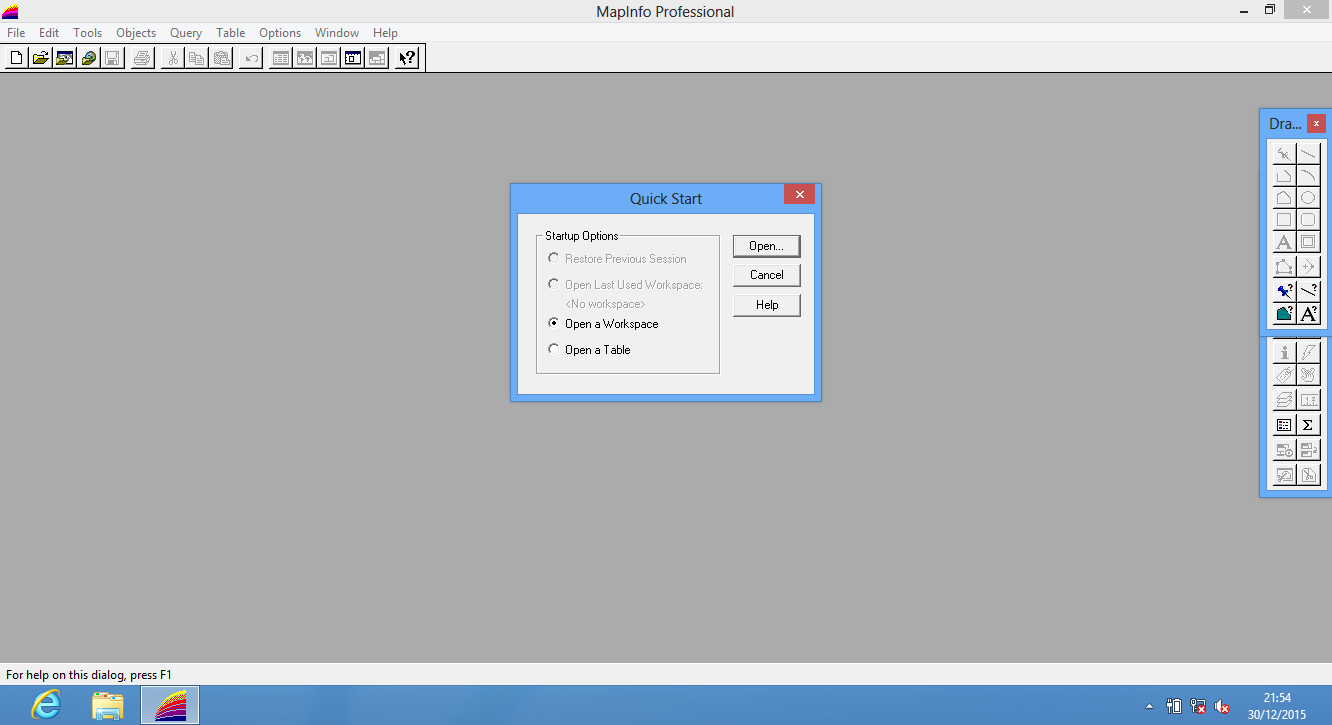
\includegraphics[width=1\textwidth]{./resources/000-start-mapinfo8}
      \caption{Jendela awal Mapinfo 8}
    \end{figure}
    
    \item Klik \textbf{Cancel} pada box \textit{Quick Start}
    
    \item Drag box \textbf{Main} dan \textbf{Standard} ke atas, tempatkan dibawah menu utama, menjadi seperti tampilan berikut :
  
    \begin{figure}[H]  
      \centering
      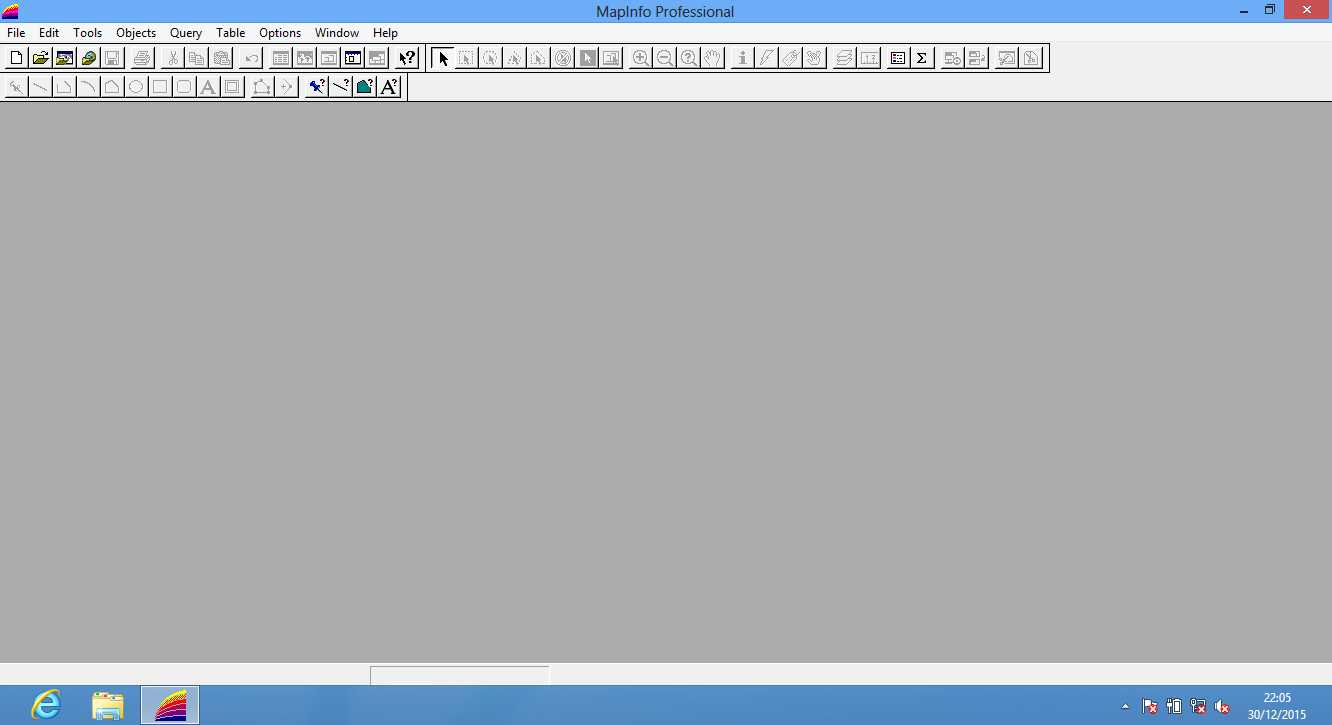
\includegraphics[width=1\textwidth]{./resources/001-rapih-icon}
      \caption{Posisi Icon Yang Telah Dirapihkan}
    \end{figure}
  
  \end{enumerate}
  
  \item \textbf{Membuat File Baru}
  
  \begin{enumerate}[1.]
  
    \item Pilih File -\textgreater New Table, sehingga muncul tampilan berikut :
    
    \begin{figure}[H]
      \centering
      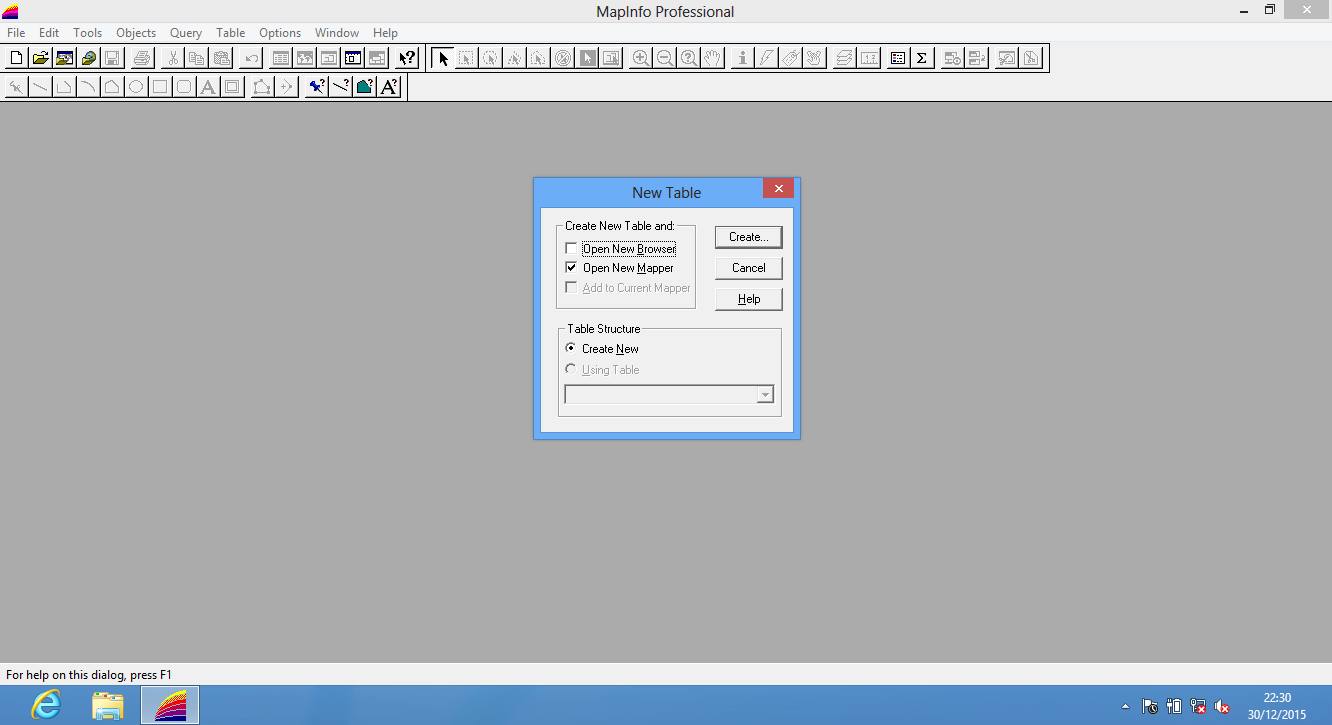
\includegraphics[width=1\textwidth]{./resources/002-new-mapper}
      \caption{Jendela Membuat File Baru}
    \end{figure}
    
    \item Kemudian tekan tombol \textbf{Create} sehingga muncul jendela berikut :
    
    \begin{figure}[H]
      \centering
	  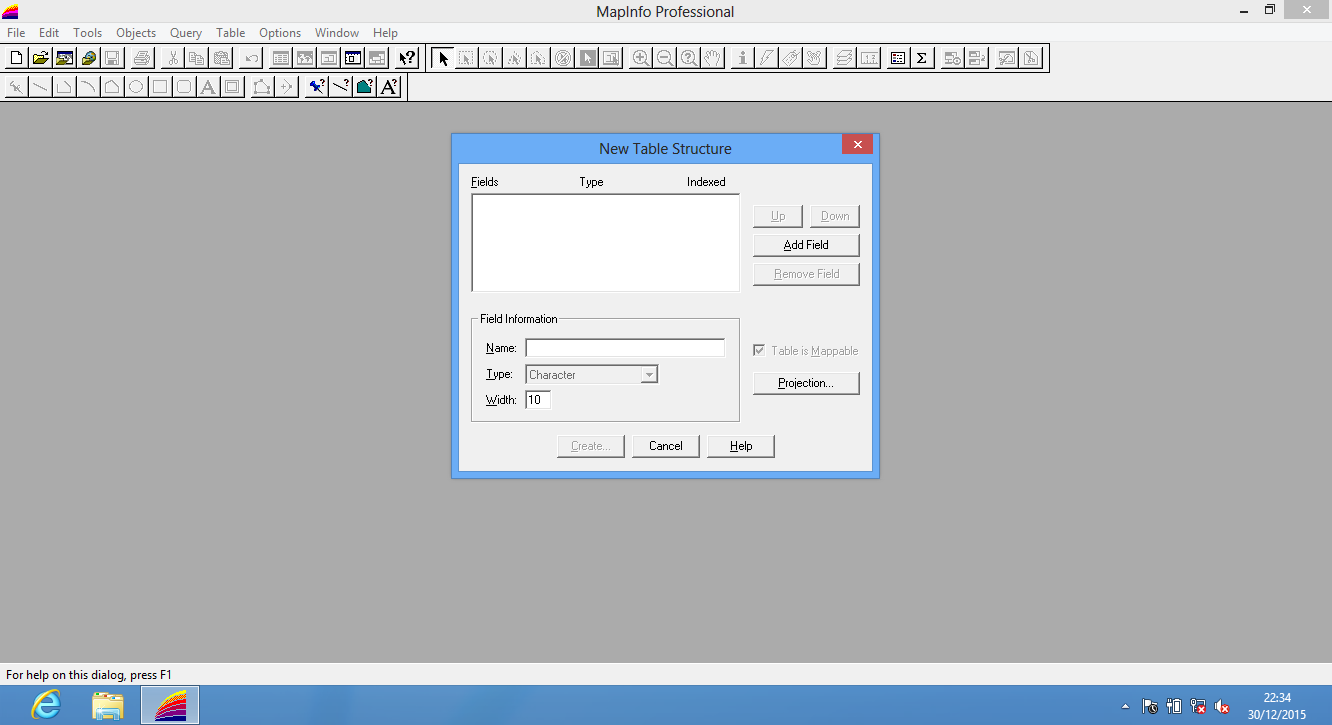
\includegraphics[width=1\textwidth]{./resources/003-pembentukan-tabel}
	  \caption{Jendela pembentukan field tabel}
	\end{figure}
    
    \item Untuk pengisian nama field, nantinya akan disesuaikan dengan jenis layer yang akan kita bangun. Sebagai contoh, apabila nanti akan membuat layer bidang, akan ada field d\_nop untuk menyimpan NOP bidangnya, apabila nanti akan membuat layer jalan, maka akan ada field d\_nm\_jln untuk menyimpan nama jalan.
    
    Sebagai referensi pembuatan field-field apa saja yang dibentuk sesuai dengan kondisi layernya, maka berikut disajikan aturan penamaan field sesuai dengan Peraturan Bupati Brebes tentang Pedoman Pendaftaran, Pendataan, Penilaian, dan Pelaporan Objek dan Subjek Pajak Bumi dan Bangunan Perdesaan dan Perkotaan di Kabupaten Brebes.
    
    \begin{enumerate}[1.]
    
      \item Layer Tanah/Bidang
      
        Layer ini berisi tanah/bidang objek pajak dalam satu Desa/Kelurahan, dimana penamaan \textit{file} mengikuti aturan 3329KKKLLL, dimana \textbf{KKK} berisi 3 (tiga) digit kode Kecamatan, dan \textbf{LLL} berisi 3 (tiga) digit kode Kelurahan/Desa.
      
        Gambar memiliki tipe \textbf{poligon}, dengan \textit{Fill Pattern} \textbf{none}, \textit{Border Style} \textbf{Garis penuh}, \textit{Color} \textbf{Black}, \textit{width} \textbf{0,17mm}
        
        \textit{Struktur basis data}
      
        \begin{tabular}{| l | c | c | p{5cm} |}
          \hline
          Nama Field & Type & Index & Keterangan \\
          \hline
          d\_nop & character(18) & index 1 & NOP setiap bidang tanah \\
          \hline
          d\_luas & decimal(10,2) & & Luas Bidang tanah dengan menggunakan update  column terhadap field \textbf{d\_luas} dengan value assist function area. \\
          \hline          
        \end{tabular}
        
      \item Layer Bangunan
      
        Layer ini berisi gambar denah bangunan dalam satu Desa/Kelurahan, dimana penamaan \textit{file} mengikuti aturan 3329KKKLLLbg, dimana \textbf{KKK} berisi 3 (tiga) digit kode Kecamatan, dan \textbf{LLL} berisi 3 (tiga) digit kode Kelurahan/Desa.
      
        Gambar memiliki tipe \textbf{poligon}, \textit{Fill Pattern} \textbf{(MapInfo No. 5)}, \textit{Foreground} \textbf{(MapInfo no. 7)}, \textit{Background} \textbf{none}, \textit{Border Style} \textbf{Garis Putus} (\textit{line style} \textbf{MapInfo No. 5}, \textit{Color} \textbf{Hijau}, \textit{width} \textbf{0,17mm}
        
        \textit{Struktur basis data}
      
        \begin{tabular}{| l | c | c | p{5cm} |}
          \hline
          Nama Field & Type & Index & Keterangan \\
          \hline
          d\_nop & character(21) & Index 1 & NOP ditambah nomor bangunan setiap bangunannya.\\
          \hline
        \end{tabular}
      
      \item Layer Jalan
      
        Layer ini berisi gambar jalan dalam satu Desa/Kelurahan, dimana penamaan \textit{file} untuk layer ini mengikuti aturan 3329KKKLLLjl, dimana \textbf{KKK} berisi 3 (tiga) digit kode Kecamatan, dan \textbf{LLL} berisi 3 (tiga) digit kode Kelurahan/Desa.
      
        Gambar memiliki tipe \textbf{Polyline}, \textit{Style} \textbf{Garis Penuh}, \textit{color} \textbf{red}, \textit{width} \textbf{0,17mm}
        
        \textit{Struktur basis data}
      
        \begin{tabular}{| l | c | c | p{5cm} |}
          \hline
          Nama Field & Type & Index & Keterangan \\
          \hline
          d\_nm\_jln & character(30) & & Nama Jalan \\
          \hline
          d\_lbr\_jln & Integer & & Lebar jalan (rata-rata lebar pada jalan tersebut) \\    
          \hline
        \end{tabular}

      
      \item Layer Sungai
      
        Layer ini berisi gambar sungai dalam satu Desa/Kelurahan, dimana penamaan \textit{file} untuk layer ini mengikuti aturan 3329KKKLLLsg, dimana \textbf{KKK} berisi 3 (tiga) digit kode Kecamatan, dan \textbf{LLL} berisi 3 (tiga) digit kode Kelurahan/Desa.
      
        Gambar memiliki tipe \textbf{polyline}, \textit{style} \textbf{Garis penuh}, \textit{color} \textbf{blue}, \textit{width} \textbf{0,17mm}
        
        \textit{Struktur basis data}
      
        \begin{tabular}{| l | c | c | p{5cm} |}
          \hline
          Nama Field & Type & Index & Keterangan \\
          \hline
          d\_nm\_sng & character(30) &  & Nama Sungai \\
          \hline
          d\_lbr\_sng & integer & & Lebar sungai (rata-rata lebar pada sungai tersebut) \\
          \hline
        \end{tabular}
      
      \item Layer Text
      
        Layer ini berisi keterangan teks dalam satu Desa/Kelurahan, penamaan \textit{file} untuk layer ini mengikuti aturan 3329KKKLLLtx, dimana \textbf{KKK} berisi 3 (tiga) digit kode Kecamatan, dan \textbf{LLL} berisi 3 (tiga) digit kode Kelurahan/Desa.
      
        \begin{tabular}{| l | c | c | p{5cm} |}
          \hline
          Nama Field & Type & Index & Keterangan \\
          \hline
          d\_text & character(30) & & Sebagai penjelas / keterangan pada bidang cetak peta \\
          \hline
        \end{tabular}
        
        kolom d\_text dapat berisi :
        
        \begin{itemize}
          \item Teks mengenai keseluruhan nama utilitas jalan, sungai, informasi nama wilayah yang bersebelahan, informasi lokasi penting, dan sebagainya, yang tidak terdapat termasuk layer-layer lain berwarna hitam dengan tipe huruf \textit{italic} berukuran sesuai dengan gambar.
          \item Batas tepi jalan diperkeras berwarna merah ukuran garis paling tipis
          \item Batas tepi jalan tidak diperkeras berwarna coklat kekuningan berukuran garis paling tipis.
          \item Batas tepi jalan TOL berwarna merah berukuran garis tipis no. 2,
          \item Batas tepi sungai berwarna biru berukuran garis tipis no.2
          \item Utilitas yang disertai dengan simbolnya.
        \end{itemize}
      
      \item Layer Batas Blok
      
        Layer ini menggambarkan batas blok dalam suatu Desa/Kelurahan, penamaan \textit{file} mengikuti aturan 3329KKKLLLbl, dimana \textbf{KKK} berisi 3 (tiga) digit kode Kecamatan, dan \textbf{LLL} berisi 3 (tiga) digit kode Kelurahan/Desa.
      
        Gambar memiliki \textit{tipe} \textbf{Polygon}, \textit{fill pattern} \textbf{None}, \textit{border style} \textbf{garis putus dan titik} (\textit{line style} \textbf{Mapinfo Nomor 13}, \textit{color} \textbf{blue}, \textit{width} \textbf{0,25mm}.
        
        \textit{Struktur Basis Data}
        
        \begin{tabular}{| l | c | c | p{5cm} |}
          \hline
          Nama Field & Type & Index & Keterangan \\
          \hline
          d\_blok & character(13) & & Kode wilayah + Nomor Blok \\
          \hline
        \end{tabular}
      
      \item Layer Simbol
      
      Layer ini digunakan untuk memberikan simbol simbol umum pada peta dalam satu Desa/Kelurahan. Penamaan \textit{file} untuk layer ini mengikuti aturan 3329KKKLLLsi, dimana \textbf{KKK} berisi 3 (tiga) digit kode Kecamatan, dan \textbf{LLL} berisi 3 (tiga) digit kode Desa/Kelurahan.
      
      \textit{Struktur Basis Data}
      
      \begin{tabular}{| l | c | c | p{5cm} |}
        \hline
        Nama Field & Type & Index & Keterangan \\
        \hline
        d\_kd\_simbol & character(4) & & Kode simbol \\
        \hline
      \end{tabular}
      
      \textit{Rincian Layer Simbol}
      
      \begin{tabular}{| c | c |}
        \hline
        Kode Simbol & Uraian Simbol \\
        \hline
        1 & Kuburan Islam \\
        \hline
        2 & Kuburan Kristen \\
        \hline
        3 & Kuburan Lainnya \\
        \hline
        4 & Masjid \\
        \hline
        5 & Gereja \\
        \hline
        6 & Candi \\
        \hline
        7 & Pura/Puri \\
        \hline
        8 & Klenteng \\
        \hline
        9 & Kantor \\
        \hline
        10 & Titik Triangulasi \\
        \hline
        11 & Tugu / Titik Poligon \\
        \hline
      \end{tabular}
      
      \item Layer Batas Kelurahan
      
      Layer ini berisi gambar batas wilayah administrasi tiap Desa/Kelurahan dalam satu Kecamatan. Penamaan \textit{file} untuk layer ini mengikuti aturan 3329KKK, dimana \textbf{KKK} berisi 3 (tiga) digit kode Kecamatan.
      
      Gambar memiliki \textit{tipe} \textbf{Polygon}, \textit{fill pattern} \textbf{none}, \textit{border style} \textbf{garis putus} (\textit{line style} \textbf{MapInfo Nomor 7}), \textit{color} \textbf{black}, \textit{width} \textbf{1 mm}.
      
      \textit{Struktur basis data} 
      
      \begin{tabular}{| l | c | c | p{5cm} |}
        \hline
        Nama Field & Type & Index & Keterangan \\
        \hline
        d\_kd\_kel & character(10) & & Kode wilayah Kelurahan \\
        \hline
        d\_nm\_kel & character(25) & & Nama Kelurahan \\
        \hline
      \end{tabular}
      
      \item Layer Batas Kecamatan
      
      Layer ini berisi gambar batas administrasi untuk tiap Kecamatan dalam 1 (satu) Kabupaten/Kota. Penamaan \textit{file} untuk layer ini hanya 3329, karena gambarnya hanya berisi batas administrasi Kecamatan di Kabupaten Brebes.
      
      Gambar memiliki \textit{tipe} \textbf{Polygon}, \textit{fill pattern} \textbf{none}, \textit{border style} \textbf{garis putus} (\textit{line style} \textbf{MapInfo Nomor 7}), \textit{color} \textbf{black}, \textit{width} \textbf{1 mm}.
      
      \textit{Struktur basis data}
      
      \begin{tabular}{| l | c | c | p{5cm} | }
        \hline
        Nama Field & Type & Index & Keterangan \\
        \hline
        d\_kd\_kec & character(7) & & Kode wilayah Kecamatan \\
        \hline
        d\_nm\_kec & character(25) & & Nama Kecamatan \\
        \hline
      \end{tabular}
      
      \item Layer Batas Kabupaten
      
      Layer ini berisi gambar batas administrasi Kabupaten, karena wilayah yang dibutuhkan hanya Kabupaten Brebes, maka hanya ada 1 (satu) \textit{file} untuk layer ini dengan nama \textit{file} diisikan 33.
      
      Gambar memiliki \textit{tipe} \textbf{polygon}, \textit{fill pattern} \textbf{none}, \textit{border style} \textbf{garis positif} (\textit{line style} \textbf{MapInfo nomor 32}), \textit{color} \textbf{black}, \textit{width} \textbf{1 mm}.
      
      \textit{Struktur basis data}
      
      \begin{tabular}{| l | c | c | p{5cm} |}
        \hline
        Nama Field & Type & Index & Keterangan \\
        \hline
        d\_kd\_dt2 & character(4) & & Kode wilayah Daerah Kabupaten \\
        \hline
        d\_nm\_dt2 & character(25) & & Nama Daerah Kabupaten \\
        \hline
      \end{tabular}
      
    \end{enumerate}
  
  \end{enumerate}
  
  \item \textbf{Membuat Layer}
  
  \begin{enumerate}[1.]
    \item Membuat \textit{workspace} baru atau membuka \textit{file} yang sudah ada.
  
    \item Pilih Map -\textgreater  Layer Control, atau cukup meng-klik ikon 
\includegraphics{./resources/004-ikon-layer-kontrol} . Sehingga akan tampil jendela berikut :
    
    \begin{figure}[H]
      \centering
      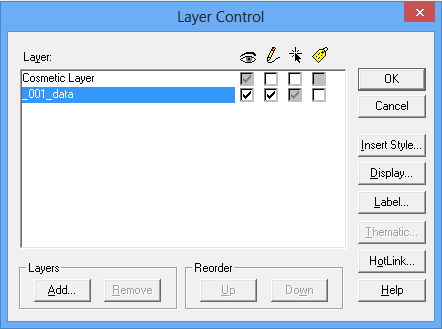
\includegraphics[width=1\textwidth]{./resources/005-jendela-layer-control}
      \caption{Jendela Layer Control}
    \end{figure}
    
    \item Pastikan bahwa file ini sudah dalam kondisi dapat di-edit. Lalu pilih \textbf{OK}. Ciri-ciri bahwa layer ini sudah dapat di-edit dapat dilihat tanda centang pada gambar berikut :
    
    \begin{figure}[H]
      \centering
      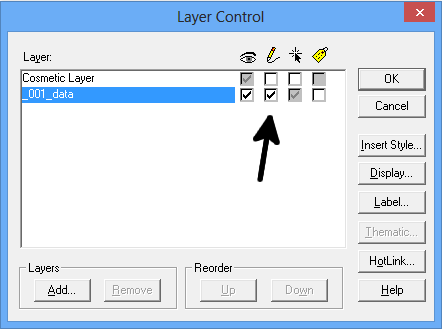
\includegraphics[width=1\textwidth]{./resources/006-mode-edited}
      \caption{Layer Dapat Diedit\label{fig:layeredited}}
    \end{figure}
    
    \item Buat objek titik, garis, atau polygon dengan meng-klik ikon-ikon berikut :
    
    \begin{figure}[H]
      \centering
      
\includegraphics[width=1\textwidth]{./resources/007-ikon-drawing}
      \caption{Ikon Untuk Membuat Objek}
    \end{figure}
    
    \item Jika selesai, simpan dengan memilih menu File -\textgreater Save Table -\textgreater Save. 
  \end{enumerate}
  
  \item \textbf{Mengedit File}
  
  \begin{enumerate}[1.]
    \item Buka \textit{file} yang sudah dibuat, atau buat layer baru, lalu pastikan \textit{file} dalam kondisi dapat di-edit dengan meng-klik Map -\textgreater Layer Control sehingga tampil jendela seperti gambar \ref{fig:layeredited}
    
    \item Pilih objek yang akan di edit dengan meng-klik ikon \textbf{select} seperti ini 
\includegraphics{./resources/008-ikon-select}
    
    \item Pilih ikon Reshape untuk menampilkan vertex, yang berbentuk seperti ini 
\includegraphics{./resources/009-ikon-reshape} klik salah satu vertex lalu tarik ke arah lain.
    
    Sebagai contoh, bentuk objek yang akan kita ubah dengan fungsi \textit{reshape} adalah seperti ini :
    
    \begin{figure}[H]
      \centering
      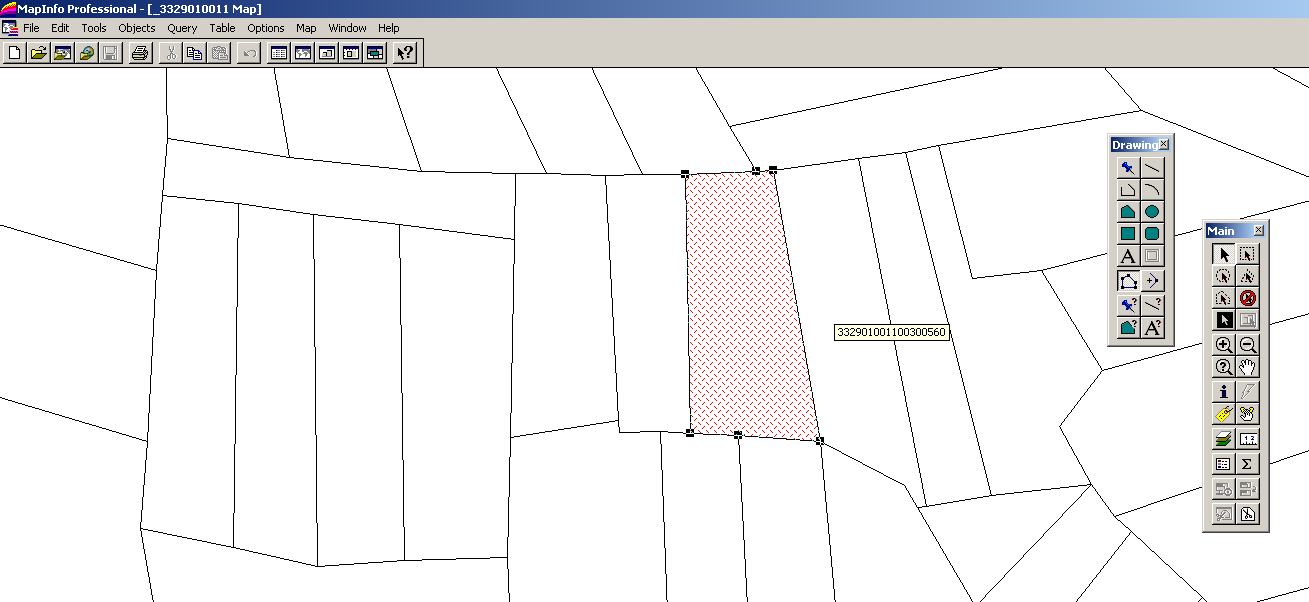
\includegraphics[width=1\textwidth]{./resources/010-sebelum-reshape}
      \caption{Bentuk Bidang Sebelum dilakukan Reshape}
    \end{figure}
    
    Dan contoh bentuk objek setelah kita ubah dengan fungsi \textit{reshape} menjadi seperti ini :
    
    \begin{figure}[H]
      \centering
      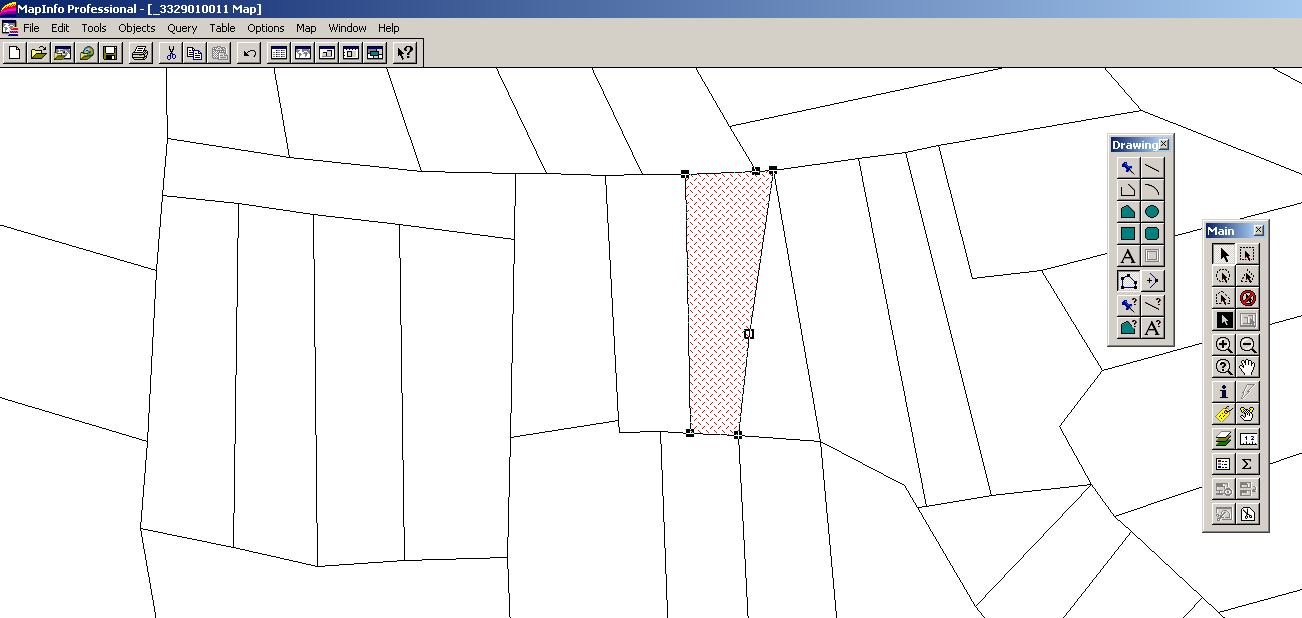
\includegraphics[width=1\textwidth]{./resources/011-sesudah-reshape}
      \caption{Bentuk Bidang Setelah dilakukan Reshape}
    \end{figure}
    
    \item Pilih ikon Add Node untuk menambah vertex. Bentuk ikonnya seperti ini 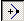
\includegraphics{./resources/012-ikon-add-node}
  \end{enumerate}
  
  \item \textbf{Operasi Penggabungan (Combine)}
  
  \begin{enumerate}[1.]
    \item Bukalah terlebih dahulu layer yang akan digabungkan objeknya, atau buat baru layer dengan dua objek yang akan digabungkan. Sebagai contoh seperti gambar berikut :
    
    \begin{figure}[H]
      \centering
      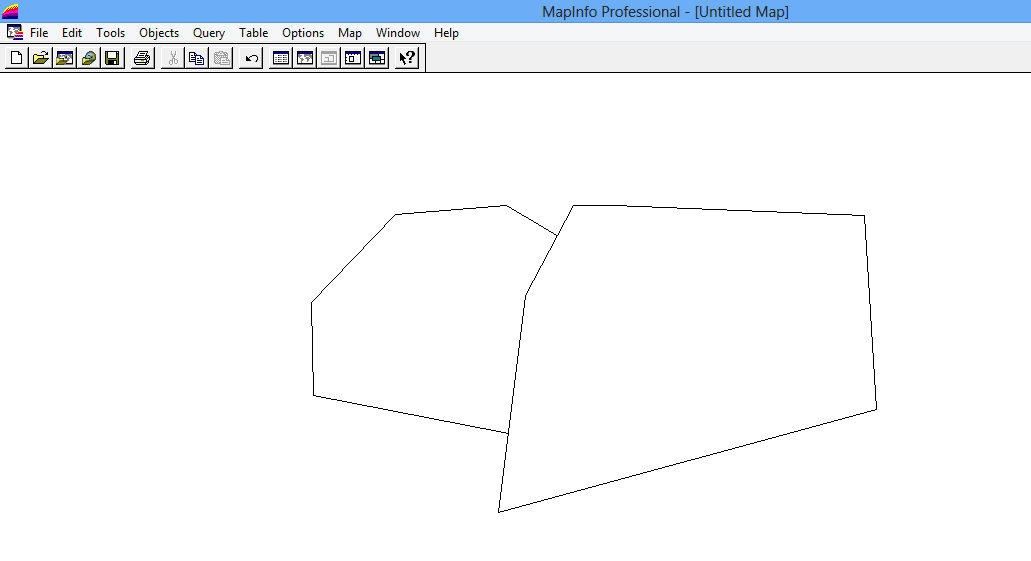
\includegraphics[width=1\textwidth]{./resources/013-layer-untuk-combine}
      \caption{Contoh Bentuk Bidang-Bidang Yang Akan Digabungkan}
    \end{figure}
    
    \item Pilih dua objek yang akan digabung dengan menggunakan ikon \textit{select} seperti ini 
\includegraphics{./resources/008-ikon-select} dengan menekan tombol Shift pada \textit{keyboard}, sehingga akan terlihat seperti gambar berikut :
    
    \begin{figure}[H]
      \centering
      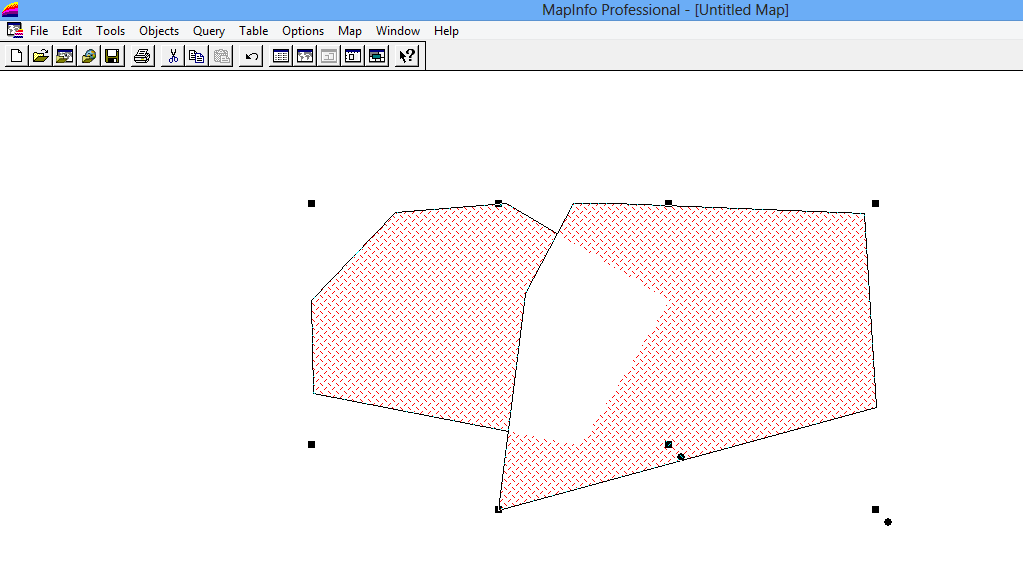
\includegraphics[width=1\textwidth]{./resources/014-dua-objek-untuk-combine}
      \caption{Contoh Bidang-Bidang Berhimpit yang Akan Digabung}
    \end{figure}
    
    Sebagai tambahan bahwa kedua bidang tersebut saling tumpang tindih, sehingga bagian bidang yang saling tumpang tindih tidak terlihat terarsir.
    
    \item Pada menu utama pilih Object -\textgreater Combine atau cukup dengan meng-klik kanan lalu pilih Combine, sehingga akan muncul jendela berikut :
    
    \begin{figure}[H]
      \centering
      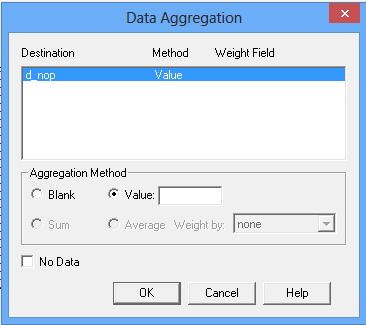
\includegraphics[width=1\textwidth]{./resources/015-window-aggregation-untuk-combine}
      \caption{Jendela Agregasi Data}
    \end{figure}
    
    Karena kedua bidang biasanya memiliki informasi atribut masing-masing, maka diperlukan kejelasan untuk penggabungan datanya pula, melalui jendela inilah kita memberikan informasi atribut untuk objek baru hasil penggabungan.
    
    \item Setelah mengisikan informasi untuk penggabungan/agregasi datanya, jika kita menekan tombol \textbf{Enter} maka kedua objek yang digabung akan terlihat seperti gambar berikut :
    
    \begin{figure}[H]
      \centering
      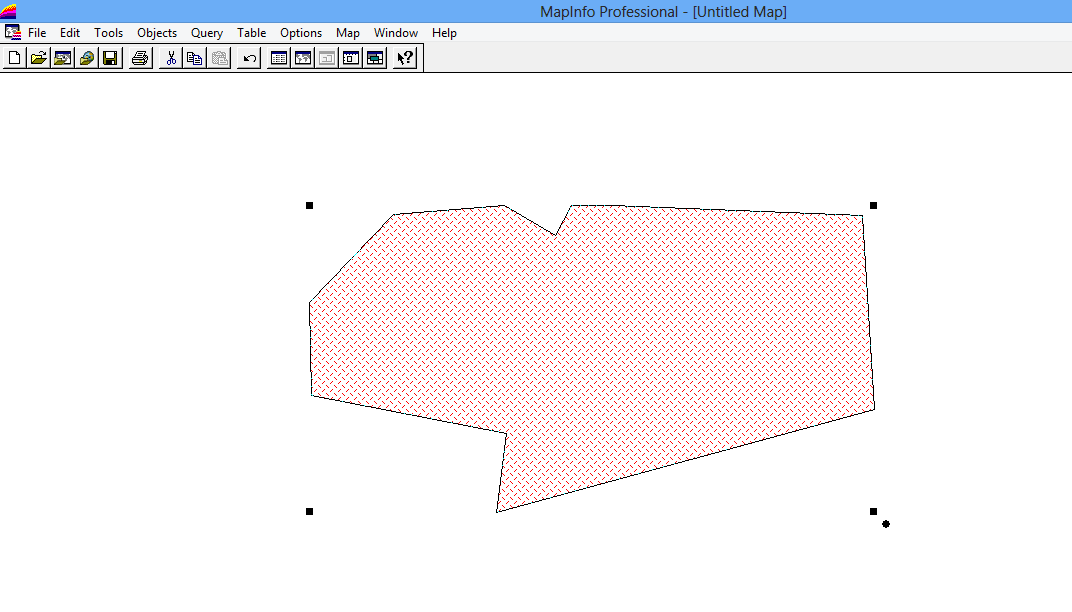
\includegraphics[width=1\textwidth]{./resources/016-objek-hasil-combine}
      \caption{Hasil Penggabungan Kedua Objek}
    \end{figure}
  \end{enumerate}
  
  \item \textbf{Operasi Pemisahan (Split)}
  
  \begin{enumerate}[1.]
    \item Buka layer objek yang akan dilakukan operasi pemisahan, atau membuat layer baru untuk objek yang akan dipisah. Sebagai contoh seperti gambar dibawah ini :
    
    \begin{figure}[H]
      \centering
      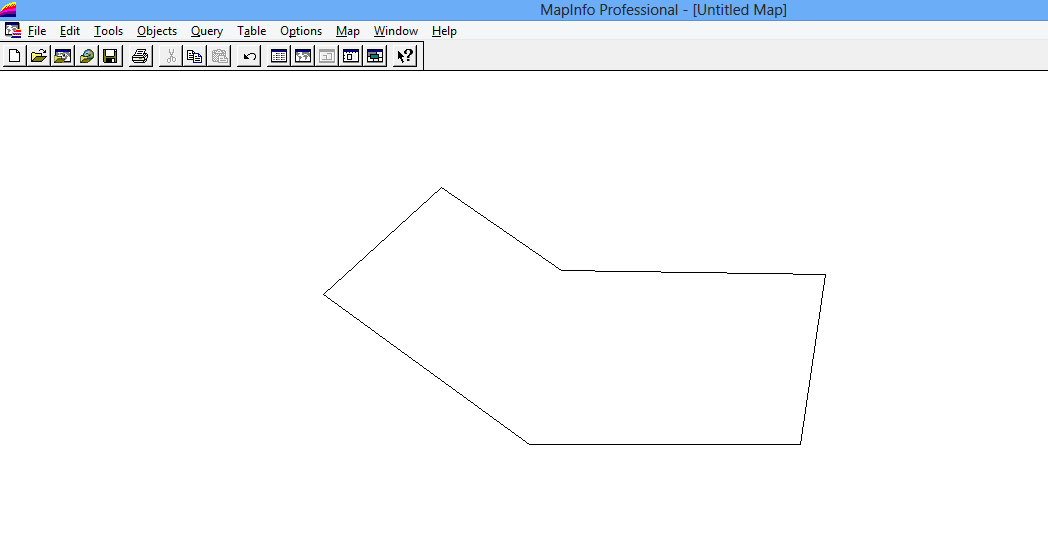
\includegraphics[width=1\textwidth]{./resources/017-layer-untuk-split}
      \caption{Objek yang akan dipisah / split}
    \end{figure}
  
    \item Pilih objek yang akan dipisah menggunakan ikon 
\includegraphics{./resources/008-ikon-select} sehingga objek akan terlihat seperti ini :
    
    \begin{figure}[H]
      \centering
      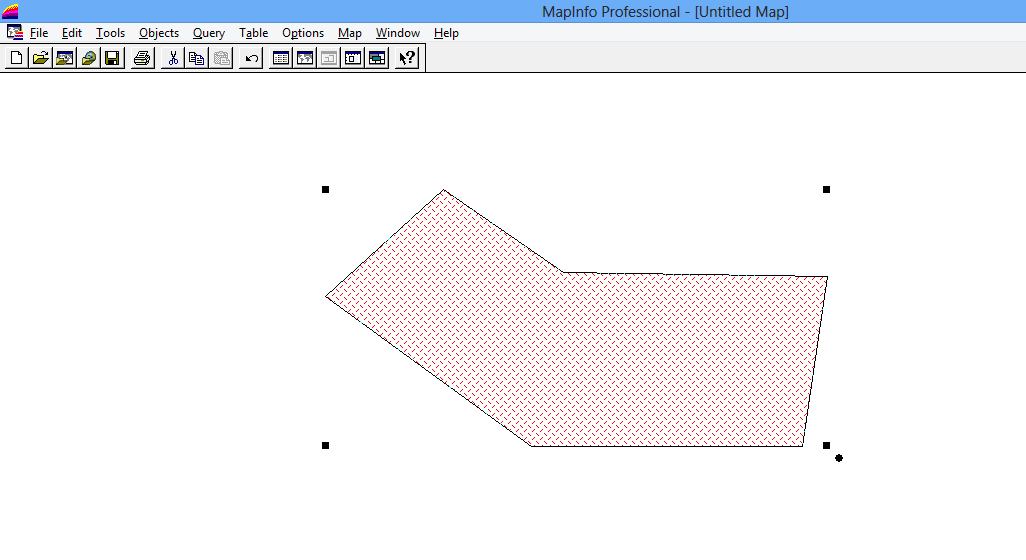
\includegraphics[width=1\textwidth]{./resources/018-objek-terpilih-untuk-split}
      \caption{Objek Yang Dipilih untuk Dipisah/Split}
    \end{figure} 
    
    \item Pilih menu Objects -\textgreater Set Target, sehingga objek menjadi terlihat seperti ini :
    
    \begin{figure}[H]
      \centering
      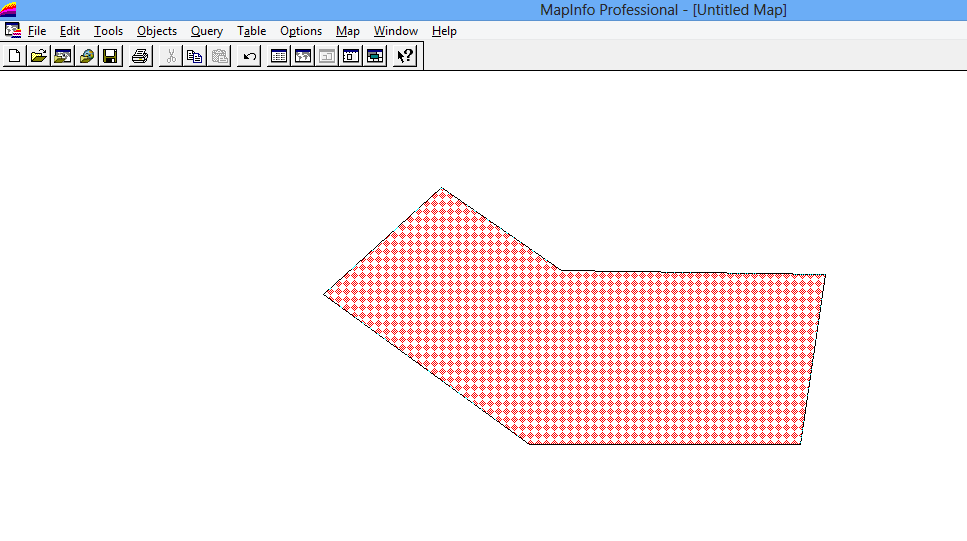
\includegraphics[width=1\textwidth]{./resources/019-objek-terpilih-set-target}
      \caption{Objek Telah Dijadikan Target Split/Pemisahan}
    \end{figure}
    
    \item Buatkan bidang poligon bantu sebagai batas pemisahan objek yang menjadi target, misalkan bidang target akan kita pisah/split menjadi 2 (dua) bagian seperti gambar berikut :
    
    \begin{figure}[H]
      \centering
      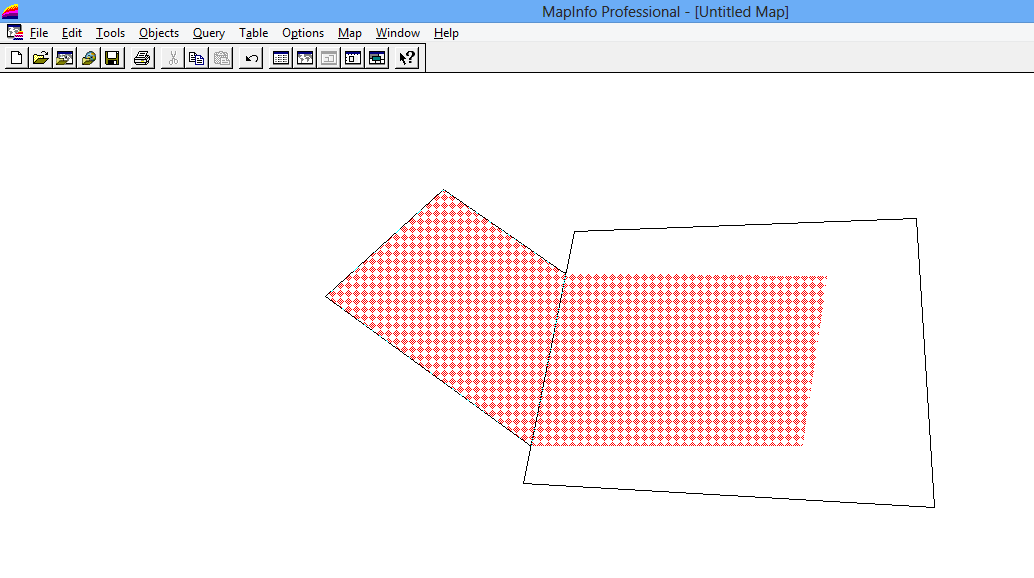
\includegraphics[width=1\textwidth]{./resources/020-poligon-pembantu-split}
      \caption{Objek Poligon Pembantu Untuk Memisahkan/Split Objek Target}
    \end{figure}
    
    \item Pilihlah objek poligon pembantu dengan ikon 
\includegraphics{./resources/008-ikon-select} sehingga objek poligon pembantu menjadi terarsir seperti ini :
    
    \begin{figure}[H]
      \centering
      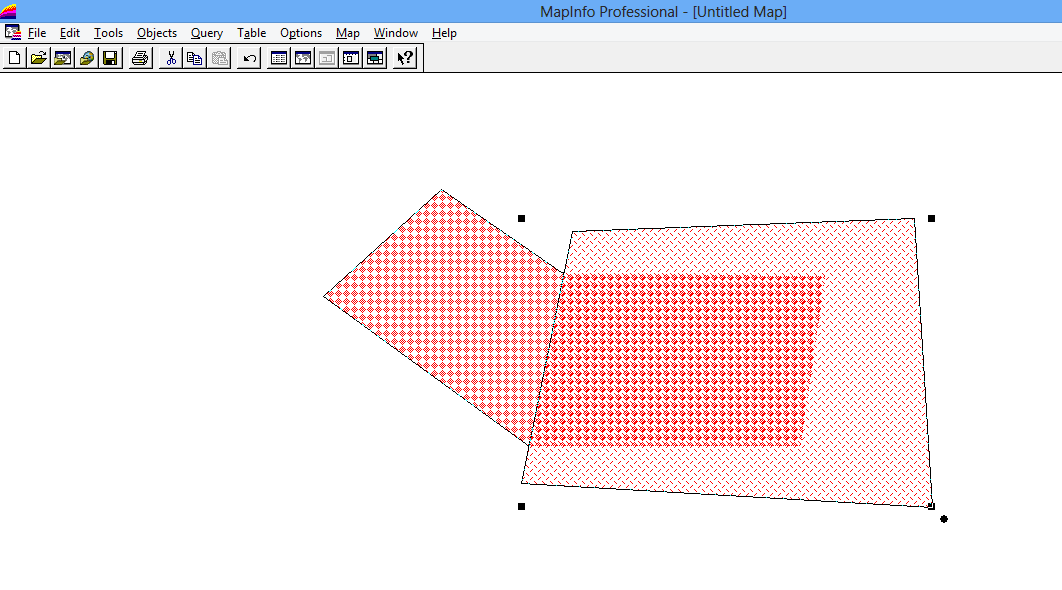
\includegraphics[width=1\textwidth]{./resources/021-poligon-pembantu-terpilih-split}
      \caption{Objek Poligon Pembantu Terpilih}
    \end{figure}
    
    \item Memilih menu Objects -\textgreater Split... sehingga muncul jendela agregasi berikut :
    
    \begin{figure}[H]
      \centering
      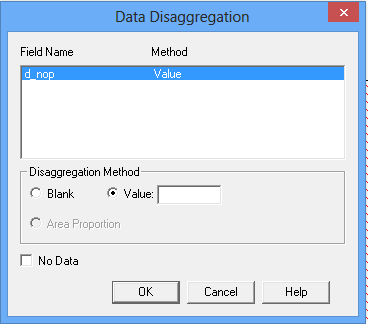
\includegraphics[width=1\textwidth]{./resources/022-window-aggregation-untuk-split}
      \caption{Jendela Aggregation Untuk Pemisahan/Split Objek}
    \end{figure}
    
    Isikan dengan data atribut baru untuk objek yang dipisah/split.
    
    \item Pilih objek poligon pembantu dengan ikon select seperti ini 
\includegraphics{./resources/008-ikon-select}, kemudian tekan tombol \textbf{delete} pada \textit{keyboard}, sehingga hasil akhir akan terlihat seperti ini :
    
    \begin{figure}[H]
      \centering
      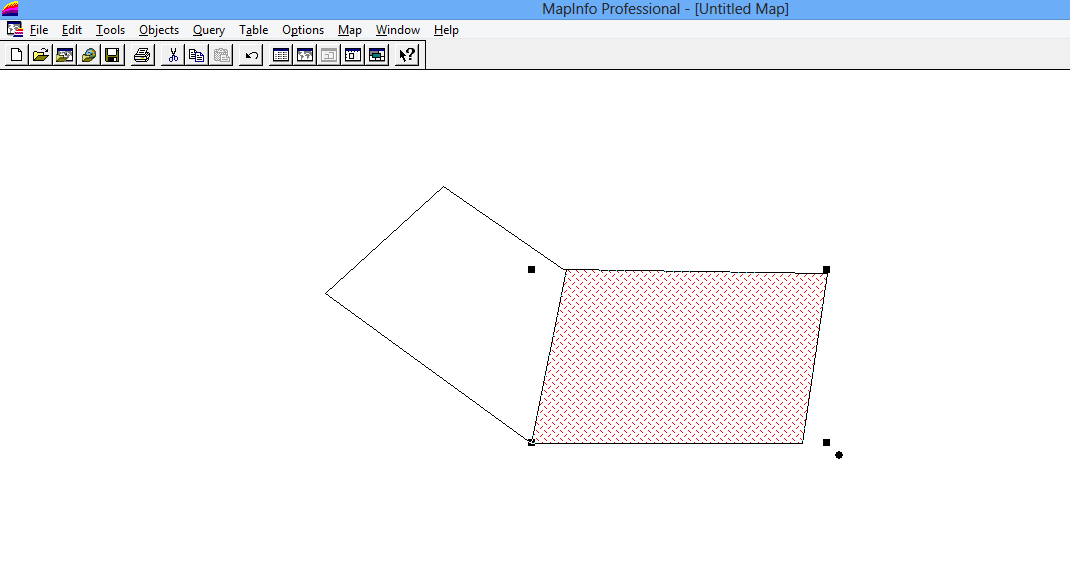
\includegraphics[width=1\textwidth]{./resources/023-objek-hasil-split}
      \caption{Hasil Akhir Operasi Pemisahan/Split}
    \end{figure}
  \end{enumerate}
  
  \item \textbf{Operasi Pemotongan 1 (Erase)}
  
  \begin{enumerate}[1.]
    \item Buka layer yang objeknya akan dilakukan pemotongan, atau buat layer baru dan gambarkan objek yang akan dilakukan operasi pemotongan 1, atau operasi pemotongan didalam. Berikut adalah contohnya :
    
    \begin{figure}[H]
      \centering
      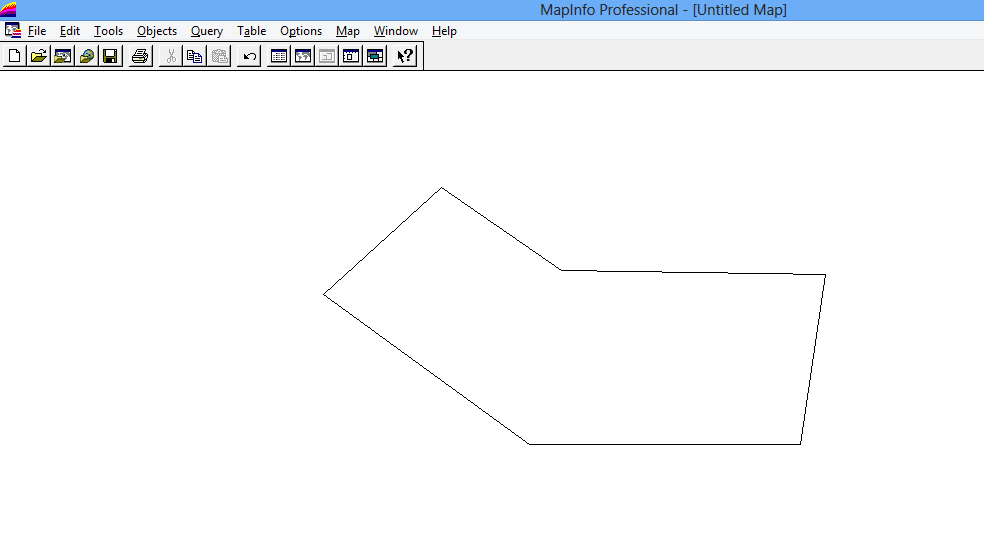
\includegraphics[width=1\textwidth]{./resources/024-layer-untuk-erase}
      \caption{Objek Yang Akan Dilakukan Pemotongan}
    \end{figure}  
  
    \item Pilih objek yang akan di potong menggunakan ikon 
\includegraphics{./resources/008-ikon-select} sehingga akan terlihat seperti berikut :
    
    \begin{figure}[H]
      \centering
      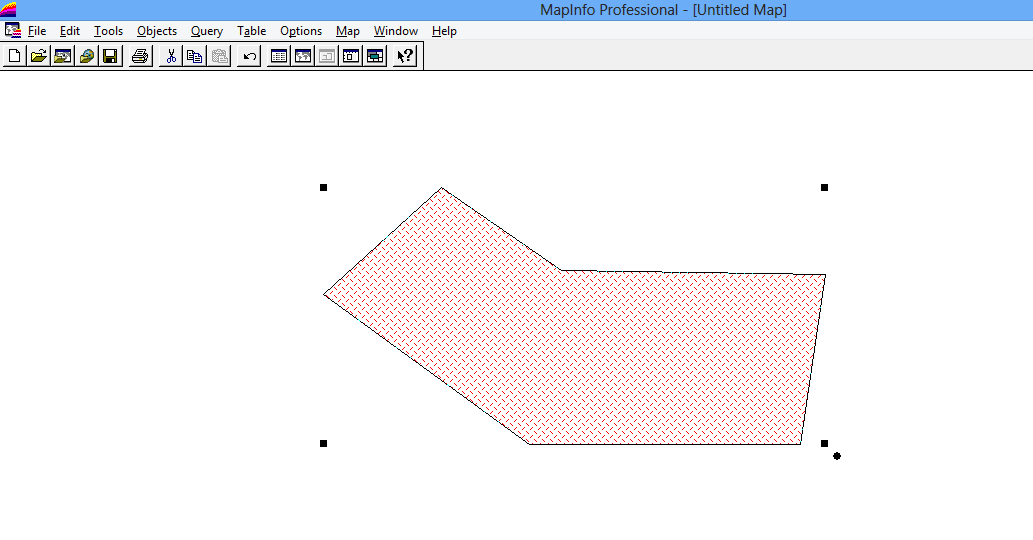
\includegraphics[width=1\textwidth]{./resources/025-objek-terpilih-untuk-erase}
      \caption{Objek Terpilih Untuk Dilakukan Operasi Penghapusan}
    \end{figure}
    
    \item Pilih menu Objects -\textgreater Set Target, sehingga objek terpilih menjadi terlihat seperti ini :
    
    \begin{figure}[H]
      \centering
      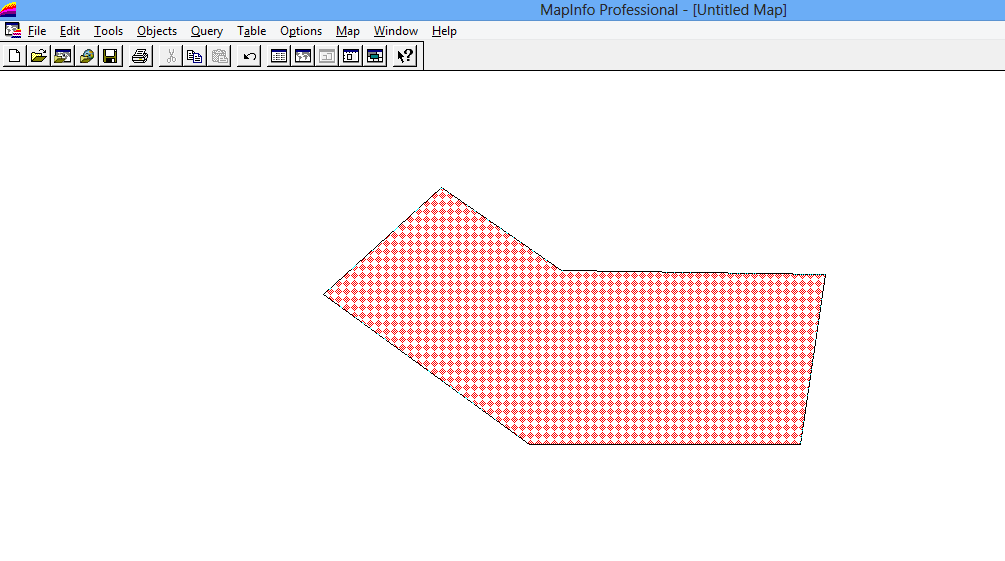
\includegraphics[width=1\textwidth]{./resources/026-objek-tertarget-untuk-erase}
      \caption{Objek Terpilih Sudah Menjadi Target Pemotongan}
    \end{figure}
    
    \item Buat polygon sebagai objek bantu untuk melakukan pemotongan, sebagai contoh seperti gambar berikut :
    
    \begin{figure}[H]
      \centering
      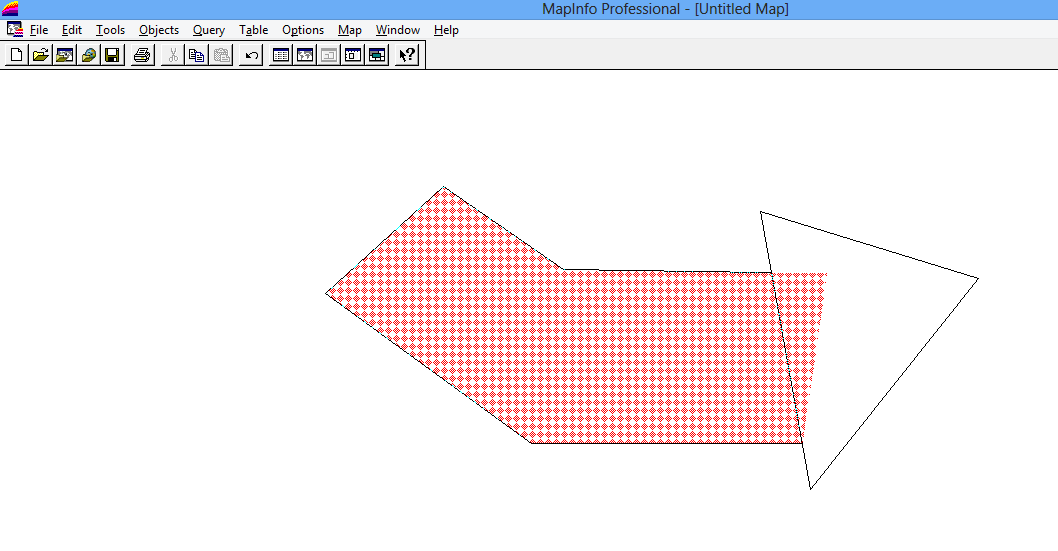
\includegraphics[width=1\textwidth]{./resources/027-objek-pembantu-erase}
      \caption{Objek Pembantu Untuk Melakukan Pemotongan}
    \end{figure}
    
    \item Pilih objek pembantu dengan menggunakan ikon select seperti ini 
\includegraphics{./resources/008-ikon-select}, sehingga objek pembantu akan terlihat seperti ini :
    
    \begin{figure}[H]
      \centering
      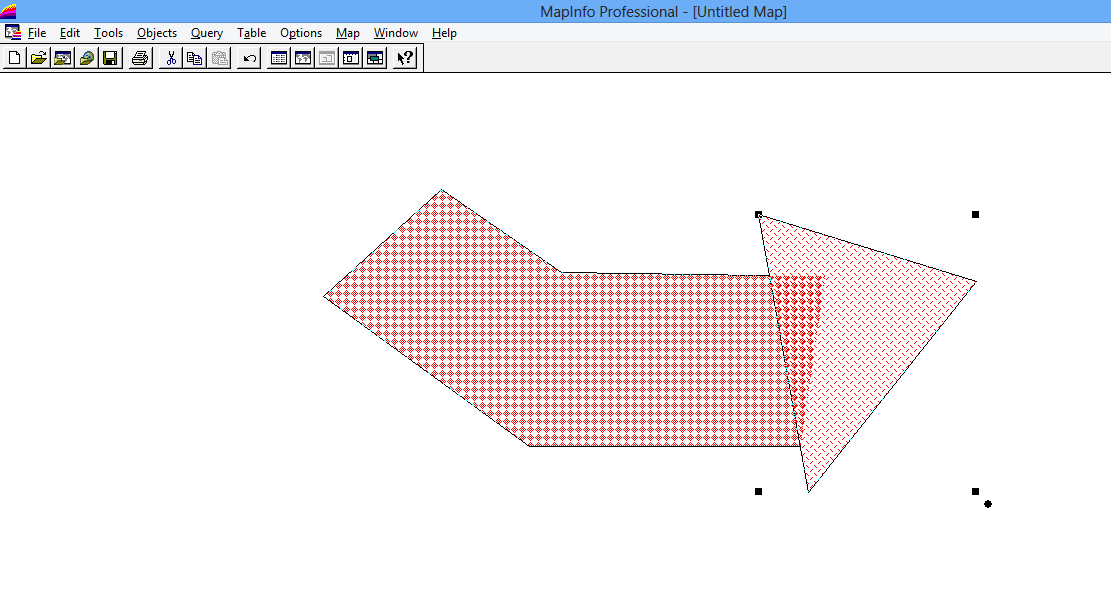
\includegraphics[width=1\textwidth]{./resources/028-objek-pembantu-erase-terpilih}
      \caption{Objek Pembantu Terpilih}
    \end{figure}
    
    \item Pilih menu Objects -\textgreater Erase untuk menghapus bagian yang ada di dalam objek pembantu. Nantinya akan muncul jendela Aggregation seperti ini :
    
    \begin{figure}[H]
      \centering
      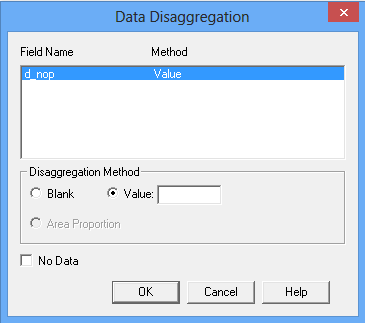
\includegraphics[width=1\textwidth]{./resources/029-window-aggregation-untuk-erase}
      \caption{Jendela Aggregation Untuk Objek Yang Tersisa}
    \end{figure}
    
    \item Setelah menekan tombol \textbf{OK} pada jendela Aggregation, maka objek sebenarnya sudah terpisah, seperti gambar berikut ini contohnya :
    
    \begin{figure}[H]
      \centering
      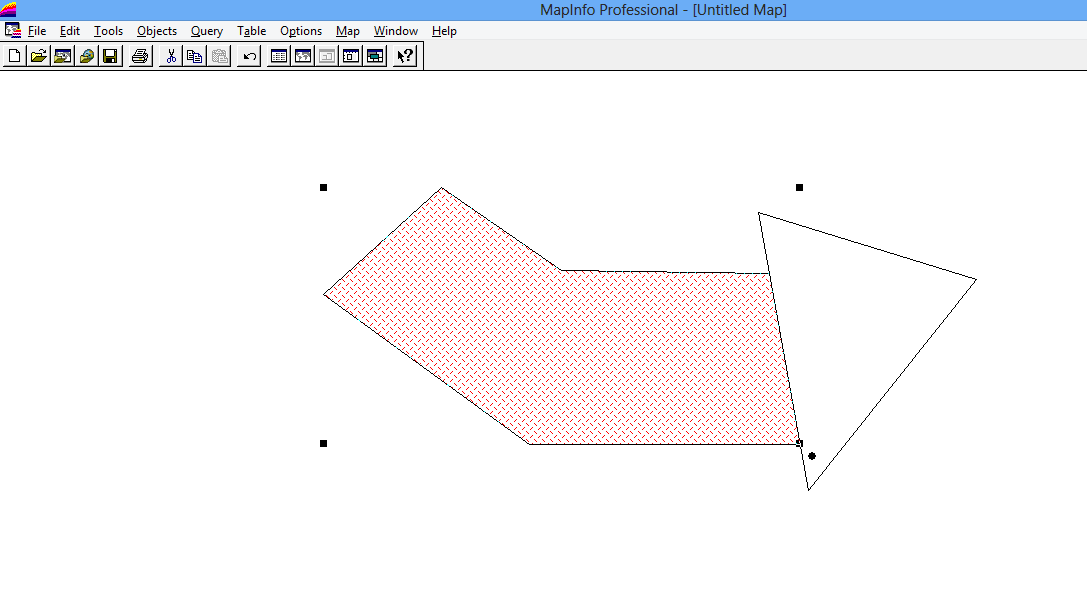
\includegraphics[width=1\textwidth]{./resources/030-objek-telah-terpotong}
      \caption{Objek Telah Terpotong}
    \end{figure}
    
    \item Hapus objek pembantu dengan ikon select 
\includegraphics{./resources/008-ikon-select}, kemudian memilih objek pembantu tersebut dan menekan tombol \textbf{delete} pada \textit{keyboard}, sehingga akan didapat hasil akhir berikut :
    
    \begin{figure}[H]
      \centering
      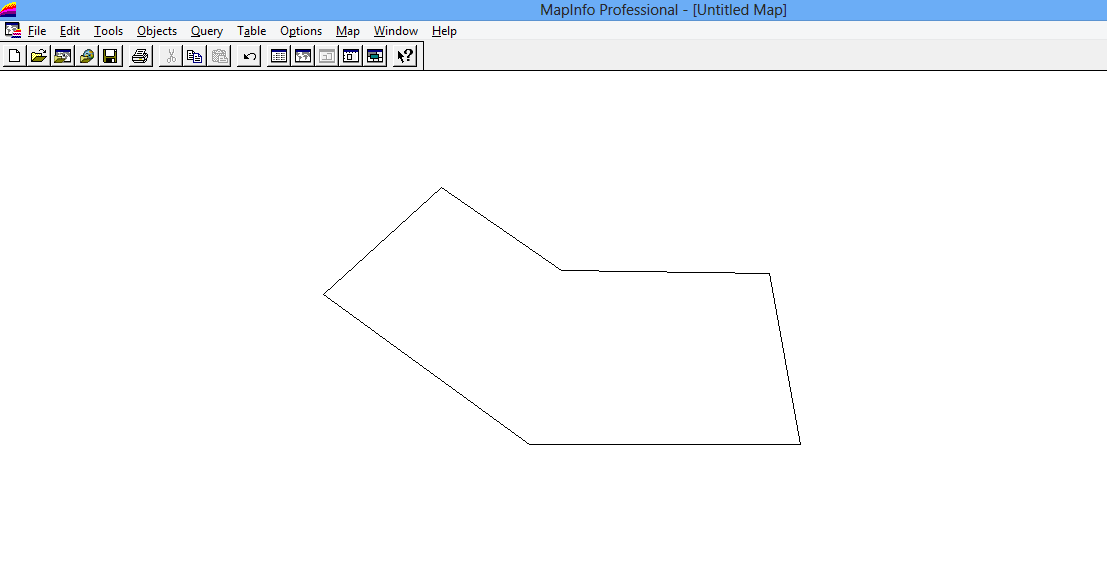
\includegraphics[width=1\textwidth]{./resources/031-hasil-akhir-erase}
      \caption{Hasil Akhir Pemotongan}
    \end{figure}
  \end{enumerate}
  
  \item \textbf{Operasi Pemotongan 2 (Erase Outside)}
  
  \begin{enumerate}[1.]
    \item Buka terlebih dahulu layer yang objeknya akan dipotong, atau buat layer baru dan buatkan objek yang akan dilakukan operasi pemotongan. Sebagai contoh seperti gambar berikut :
    
    \begin{figure}[H]
      \centering
      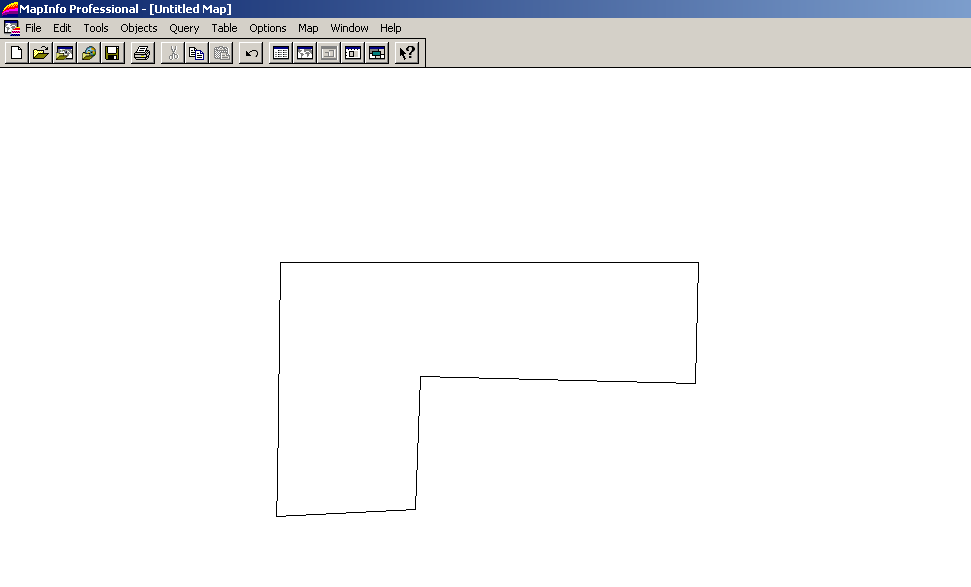
\includegraphics[width=1\textwidth]{./resources/032-layer-untuk-erase-2}
      \caption{Layer Objek Yang Akan Dipotong}
    \end{figure}
  
    \item Pilih objek yang akan di potong dengan menggunakan ikon 
\includegraphics{./resources/008-ikon-select} sehingga objek akan terlihat seperti ini :
    
    \begin{figure}[H]
      \centering
      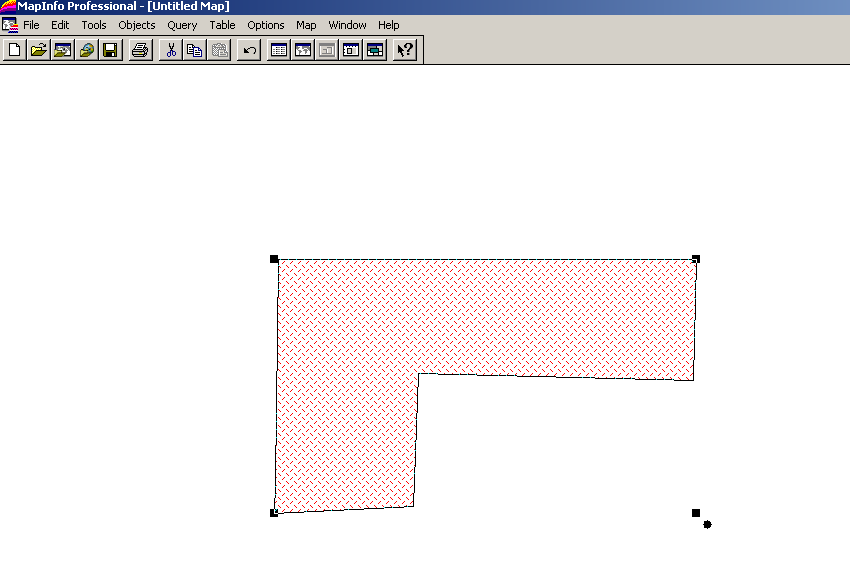
\includegraphics[width=1\textwidth]{./resources/033-objek-terpilih-untuk-erase-2}
      \caption{Objek Yang Terpilih Untuk Dilakukan Pemotongan}
    \end{figure}
    
    \item Pilih menu Objects -\textgreater Set Target sehingga objek yang akan dipotong terlihat seperti ini :
    
    \begin{figure}[H]
      \centering
      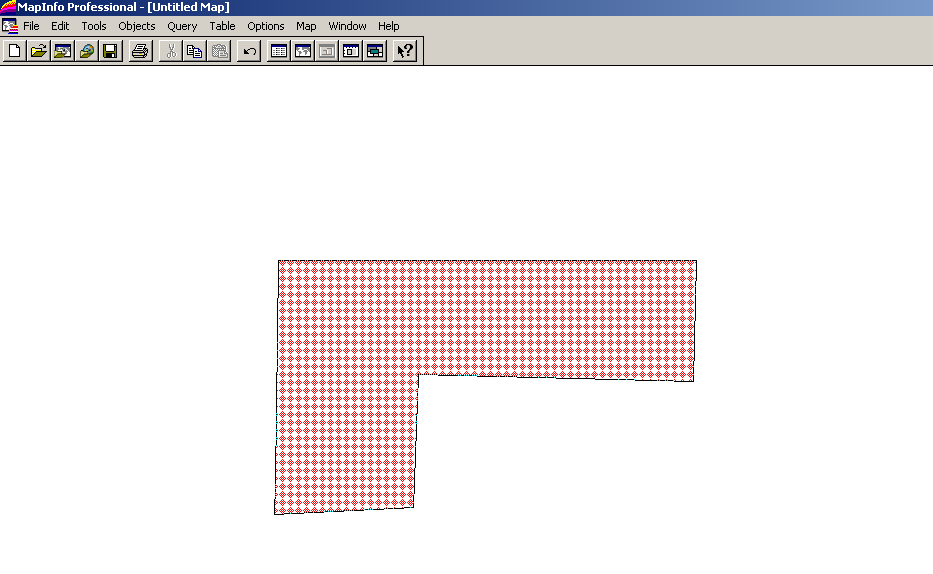
\includegraphics[width=1\textwidth]{./resources/034-objek-tertarget-untuk-erase-2}
      \caption{Objek Tertarget Untuk Dilakukan Pemotongan}
    \end{figure}
    
    \item Buat objek poligon bantuan untuk melakukan pemotongan objek, nantinya objek diluar poligon bantuan ini akan terhapus, sebagai contoh seperti gambar berikut :
    
    \begin{figure}[H]
      \centering
      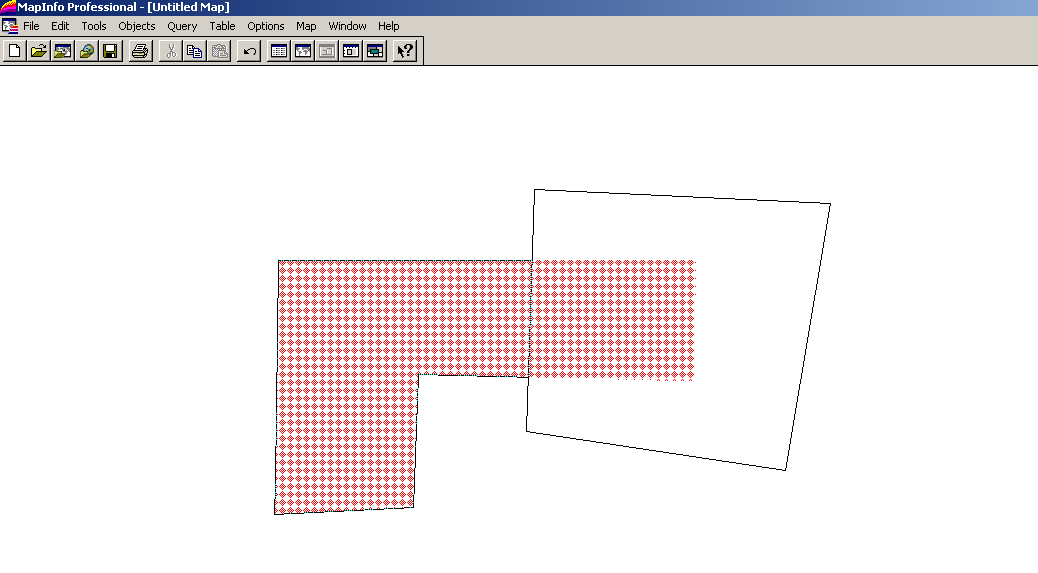
\includegraphics[width=1\textwidth]{./resources/035-poligon-bantuan-untuk-erase-2}
      \caption{Objek Poligon Bantuan Untuk Melakukan Pemotongan}
    \end{figure}
    
    \item Pilih objek poligon bantuan dengan menggunakan ikon 
\includegraphics{./resources/008-ikon-select}, sehingga objek tersebut akan terlihat seperti ini :
    
    \begin{figure}[H]
      \centering
      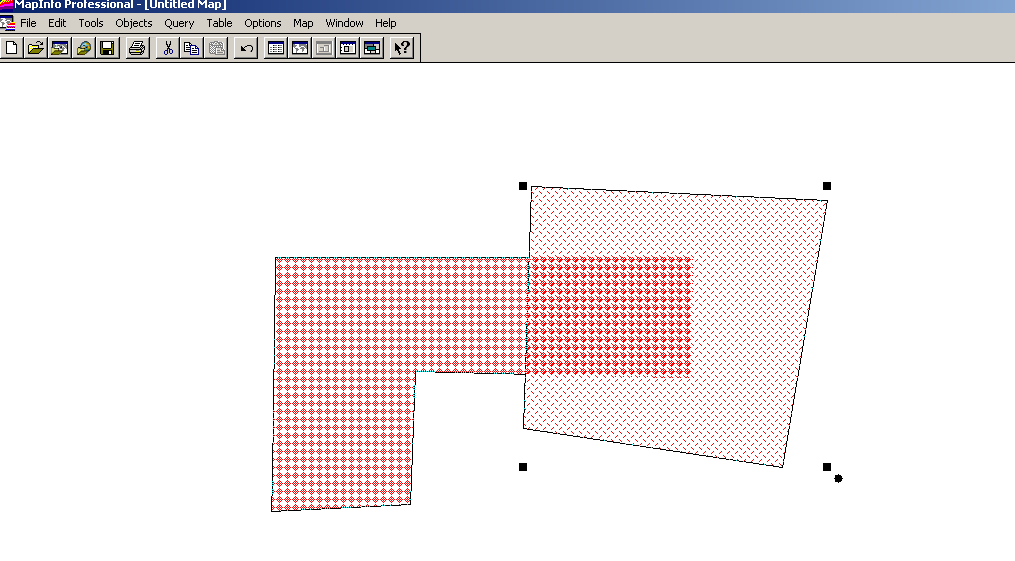
\includegraphics[width=1\textwidth]{./resources/036-poligon-bantuan-terpilih-untuk-erase-2}
      \caption{Objek Poligon Bantuan Terpilih}
    \end{figure}
    
    \item Memilih menu Objects -\textgreater Erase Outside..., sehingga muncul jendela aggregate seperti ini :
    
    \begin{figure}[H]
      \centering
      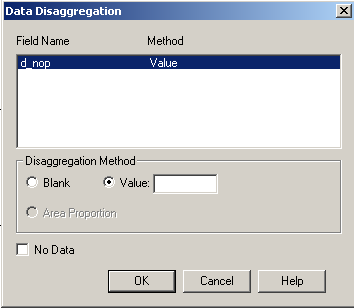
\includegraphics[width=1\textwidth]{./resources/037-jendela-aggregate-untuk-erase-2}
      \caption{Jendela Aggregate Untuk Pemotongan}
    \end{figure}
    
    Isiannya adalah berupa atribut data untuk objek yang nantinya masih tersisa.
    
    \item Setelah dilakukan pengisian atribut data untuk objek yang terpisah, hasilnya akan terlihat seperti gambar berikut :
    
    \begin{figure}[H]
      \centering
      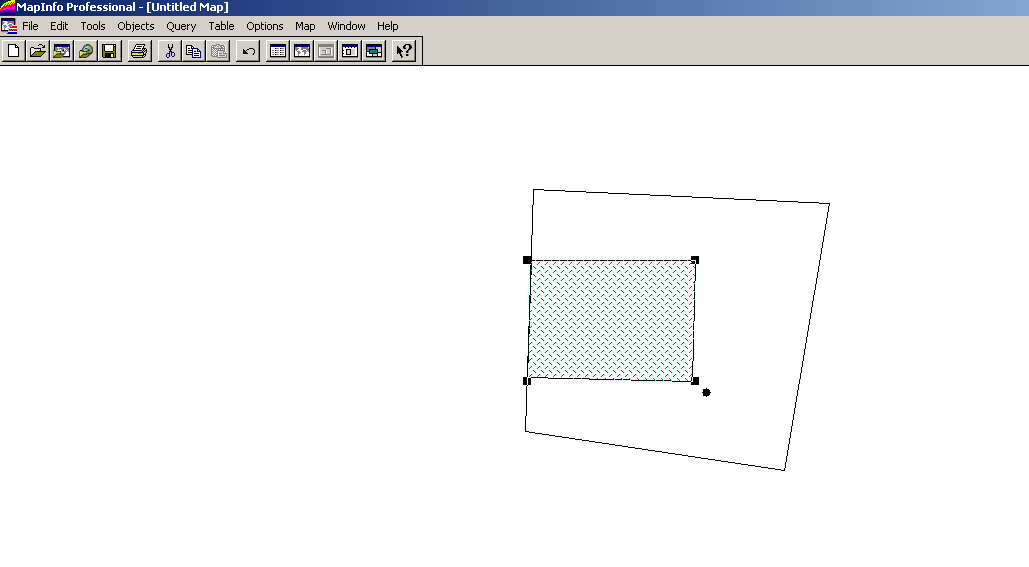
\includegraphics[width=1\textwidth]{./resources/038-objek-target-terpotong-erase-2}
      \caption{Objek Yang Masih Tersisa Dari Hasil Pemotongan}
    \end{figure}
    
    \item Pilih objek poligon bantuan dengan menggunakan ikon 
\includegraphics{./resources/008-ikon-select}, kemudian tekan tombol \textbf{delete} pada \textit{keyboard}, sehingga menghasilkan objek seperti gambar di bawah ini :
    
    \begin{figure}[H]
      \centering
      \includegraphics[width=1\textwidth]{./resources/039-hasil-erase-2}
      \caption{Hasil Akhir Pemotongan}
    \end{figure}
  \end{enumerate}
  
  \item \textbf{Menyambung Vertex (Snap)}
  
  \begin{enumerate}[1.]
    \item Buka layer yang objeknya saling terpisah atau bertumpukan kemudian akan disambungkan / dihimpitkan, atau sebagai contoh dapat membuat layer baru untuk hal ini seperti contoh gambar berikut :
    
    \begin{figure}[H]
      \centering
      \includegraphics[width=1\textwidth]{./resources/040-layer-sambung-vertex}
      \caption{Contoh Dua Objek Yang Akan Disambungkan}
    \end{figure}
    
    \item Pilih objek yang akan disambung dengan menggunakan ikon select \includegraphics{./resources/008-ikon-select}, sehingga objek akan terlihat seperti gambar berikut :
    
    \begin{figure}[H]
      \centering
      \includegraphics[width=1\textwidth]{./resources/041-objek-reshape-terpilih}
      \caption{Objek Yang Terpilih Untuk Dilakukan Reshape Penyambungan}
    \end{figure}
    
    \item Tekan huruf S pada \textit{keyboard}. Perhatikan tanda Snap yang muncul di bagian bawah jendela MapInfo yang menandakan, berarti Snap aktif. Untuk menonaktifkan Snap, tekan S kembali. Aktifnya fungsinya snap ini ditandai seperti gambar berikut :
    
    \begin{figure}[H]
      \centering
      \includegraphics[width=1\textwidth]{./resources/042-snap-aktif}
      \caption{Tanda Tombol Snap Aktif}
    \end{figure}
    
    \item Pilih ikon \textit{reshape} \includegraphics{./resources/043-ikon-reshape}, dan pindahkan titik-titik objek agar berhimpit/menyambung seperti gambar berikut :
    
    \begin{figure}[H]
      \centering
      \includegraphics[width=1\textwidth]{./resources/044-reshape-snap-ke-objek-lain}
      \caption{Hasil Reshape Objek}
    \end{figure}
  \end{enumerate}

\end{enumerate} 
\chapter{KOORDINAT}

Koordinat atau alamat keberadaan/posisi suatu wilayah dijabarkan ke dalam angka. Koordinat yang sering digunakan ada 2 (dua) jenis, yaitu koordinat geografi dan koordinat UTM (Universal Transversal Mercator).

\begin{itemize}
  \item Contoh koordinat Geografi
  
  X = $108^{\circ}30'50"; Y=7^{\circ}30'50"$
  
  \item Contoh Koordinat UTM
  
  X = 480000; Y=9800000
\end{itemize}

Datum titik nadir (konstanta/ketetapan), bumi bentuknya bulat sedangkan derajat/geografi di jabarkan di bidang datar dengan dibuat grid dan diberikan nomor. Tahun survey terbaru adalah tahun 1984 sehingga dikenal dengan \textbf{WGS1984}.

Pemilihan proyeksi \textbf{WGS1984} dilakukan dengan memilih menu Map -\textgreater Options, sehingga akan muncul jendela berikut :

\begin{figure}[H]
  \centering
  \includegraphics[width=1\textwidth]{./resources/045-jendela-map-option}
  \caption{Jendela Map Options}
\end{figure}

Kemudian klik \textbf{Projection}, sehingga muncul jendela \textit{projection} seperti berikut :

\begin{figure}[H]
  \centering
  \includegraphics[width=1\textwidth]{./resources/046-jendela-projection}
  \caption{Jendela Projection}
\end{figure}

Terakhir memilih Kategori \textbf{Universal Transverse Mercator (WGS 84)}, kemudian memilih UTM Zone 49 pada Category Members dan menekan tombol \textbf{OK}, karena posisi Kabupaten Brebes berada pada Zona 49 UTM/WGS84, seperti gambar berikut :

\begin{figure}[H]
  \centering
  \includegraphics[width=1\textwidth]{./resources/047-pemilihan-utm-wgs84}
  \caption{Pemilihan UTM WGS 84 Zona 49 S}
\end{figure}
\chapter{REGISTRASI DAN TRANSFORMASI KOORDINAT}

\begin{enumerate}[1.]
  \item Pilih File -\textgreater Open
  
  \item Cari file \textbf{peta} yang berbentuk gambar, seperti misalnya gambar dengan format \textbf{tif}, caranya, pilih \textbf{Files of Types} -\textgreater \textbf{Raster Image} seperti tampilan jendela berikut ini :
  
  \begin{figure}[H]
    \centering
    \includegraphics[width=1\textwidth]{./resources/048-membuka-file-raster}
    \caption{Jendela Untuk Membuka File Raster}.
  \end{figure}
  
  \item Buka \textit{file} \textbf{peta} tersebut sehingga muncul jendela pernyataan bahwa gambar yang akan dibuka belum terregistrasi, kemudian pilih \textbf{Register}. Jendelanya akan tampil seperti ini :
  
  \begin{figure}[H]
    \centering
    \includegraphics[width=1\textwidth]{./resources/049-a-jendela-register}
    \caption{Jendela Pernyataan Register}
  \end{figure}
  
  \item Pilih \textbf{Projection} sehingga muncul jendela \textit{image registration} seperti ini :
  
  \begin{figure}[H]
    \centering
    \includegraphics[width=1\textwidth]{./resources/051-jendela-image-registration}
    \caption{Jendela Image Registration}
  \end{figure}
    
  \item Masukan koordinat pertama pada titik GCP ke-satu dengan meng-klik \textbf{Add}. Lakukan hal yang sama pada titik-titik GCP berikutnya dilakukan searah jarum jam. Perhatikan Error RMS-nya. Edit Image X dan Image Y-nya sampai pada kolom Error menjadi 0. Perlu juga dilakukan perumusan dari koordinat yang ada pada data raster menjadi data UTM.
\end{enumerate}

 
\chapter{MEMBANGUN TOPOLOGI (Digitasi On-Screen)}

\begin{enumerate}[\bfseries A.]
  \item \textbf{Digitasi Objek Titik (Point)}
  
  \begin{enumerate}[1.]
    \item Buka file peta dengan memilih File -\textgreater Open, atau membuat layer baru untuk menyimpan titik-titik yang akan dibuat. Biasanya objek titik akan menandakan bidang tertentu tergantung gambar simbol yang dihasilkan.
    
    \item Pilih Map -\textgreater Layer Control atau cukup dengan mengklik ikon \includegraphics{./resources/052-a-ikon-layer-control} sehingga muncul jendela seperti gambar berikut :
    
    \begin{figure}[H]
      \centering
      \includegraphics[width=1\textwidth]{./resources/052-jendela-layer-control}
      \caption{Jendela Layer Control}
    \end{figure}
    
    \item Pastikan peta yang akan di digitasi dapat di-edit, perhatikan pada jendela layer control seperti yang ditunjuk tanda panah pada gambar berikut :
    
    \begin{figure}[H]
      \centering
      \includegraphics[width=1\textwidth]{./resources/052-b-kondisi-editable}
      \caption{Layer Dapat Diedit}
    \end{figure}
    
    \item Setelah selesai dengan urusan layer, sekarang kita konfigurasi simbolnya, pilih ikon \includegraphics{./resources/054-ikon-setting-simbol} sehingga muncul jendela berikut :
    
    \begin{figure}[H]
      \centering
      \includegraphics[width=1\textwidth]{./resources/055-jendela-setting-simbol}
      \caption{Jendela Setting Simbol}
    \end{figure}
    
    Kita dapat mengubah jenis huruf dan jenis simbol yang akan digunakan, termasuk disana mengubah ukuran huruf agar dapat ditampilkan lebih jelas.
    
    \item Siap untuk men-digitasi data titik (misal objek Tower BTS atau objek Pelabuhan) dengan menggunakan ikon \includegraphics{./resources/053-ikon-simbol} seperti gambar berikut :
    
    \begin{figure}[H]
      \centering
      \includegraphics[width=1\textwidth]{./resources/056-contoh-simbol}
      \caption{Contoh Penggambaran Objek Titik}
    \end{figure}
    
    \item Setelah semua data titik selesai di digitasi, simpan data dengan memilih File -\textgreater Save table.
  \end{enumerate}
  
  \item \textbf{Digitasi Objek Garis (Line)}
  
  \begin{enumerate}[1.]
    \item Tambahkan layer bila perlu untuk membuat objek garis (misal objek jalan, atau objek sungai), atau gunakan layer yang sudah ada untuk membuat objek garis.
    
    \item Pilih ikon \includegraphics{./resources/057-a-ikon-setting-garis} sehingga muncul jendela untuk dikonfigurasi sesuai kebutuhan, berikut tampilannya :
    
    \begin{figure}[H]
      \centering
      \includegraphics[width=1\textwidth]{./resources/058-jendela-setting-garis}
      \caption{Jendela Konfigurasi Objek Garis}
    \end{figure}
    
    Konfigurasinya meliputi bentuk garis yang akan dibuat, warna yang akan dipilih, serta ukuran ketebalan garis.
    
    \item Siap untuk mendigitasi data garis dengan ikon berikut :
    
    \begin{figure}[H]
      \centering
      \includegraphics[width=0.5\textwidth]{./resources/059-ikon-garis}
      \caption{Ikon Untuk Menggambar Garis}
    \end{figure}
    
    Untuk menggambar garis sendiri ada 3 (tiga) ikon yang dapat digunakan, yang pertama digunakan untuk menggambar sebuah garis lurus, yang kedua untuk menggambar beberapa garis dalam satu proses (\textit{polyline}), awal pembentukan garis dengan klik kiri, jika ingin mengakhiri pembuatan garisnya, klik ganda tombol kiri \textit{mouse}. Ikon yang ketiga yaitu menggambar garis lengkung.
    
    \item Contoh gambar yang dihasilkan dari ketiga ikon tersebut dapat dilihat pada gambar berikut :
    
    \begin{figure}[H]
      \centering
      \includegraphics[width=1\textwidth]{./resources/060-contoh-garis}
      \caption{Contoh Hasil Objek Garis}
    \end{figure}
    
    \item Setelah semua data garis selesai digitasi, simpan data dengan memilih \textbf{File} -\textgreater \textbf{Save table}.
  \end{enumerate}
  
  \item \textbf{Digitasi Objek Area (Polygon)}
  
  \begin{enumerate}[1.]
    \item Tambahkan layer bila perlu untuk membuat objek poligon, (misal objek batas Kecamatan, atau objek bidang tanah).
    
    \item Pilih ikon \includegraphics{./resources/061-ikon-setting-poligon} sehingga muncul jendela konfigurasi poligon seperti gambar berikut :
    
    \begin{figure}[H]
      \centering
      \includegraphics[width=1\textwidth]{./resources/062-jendela-setting-poligon}
      \caption{Jendela Setting Poligon}
    \end{figure}
    
    Kita dapat mengkonfigurasi beberapa hal seperti warna dan jenis isian/arsiran, jenis dan warna garis pinggir, termasuk ketebalan garis pinggir yang akan ditampilkan.
    
    \item Selanjutnya melakukan digitasi data area dengan menggunakan ikon \includegraphics{./resources/063-ikon-poligon}. Cara penggambarannya sama dengan menggambar polyline, klik satu kali di awal titik, dan akhiri dengan klik ganda di titik terakhir.
    
    \item Setelah semua data area sudah selesai digitasi, simpan data dengan memilih Map -\textgreater Save Cosmetic Object. Berikut contoh hasil jadi dari penggambaran objek bidang :
    
    \begin{figure}[H]
      \centering
      \includegraphics[width=1\textwidth]{./resources/064-hasil-poligon}
      \caption{Contoh Hasil Akhir Penggambaran Objek Area}
    \end{figure}
    
    \item Setelah semua selesai, pilih File -\textgreater Save table.
  \end{enumerate}
  
  \item \textbf{Editing Objek (Feature)}
  
  Untuk meng-edit \textit{feature} setiap objek (biasanya hanya untuk objek garis dan area saja. Objek titik tidak perlu di edit), gunakan prinsip-prinsip dasar pemetaan seperti pada \textbf{BAB 2 PENGENALAN SOFTWARE} sebelumnya. Pastikan \textit{file} yang akan diubah dalam kondisi dapat ter-edit.
\end{enumerate} 
\chapter{QUERY}

Karena data-data peta pada MapInfo selain berbentuk data spasial, adapula data yang berbentuk atribut seperti misal kolom d\_nop pada tabel layer bidang/bumi yang menyimpan informasi Nomor Objek Pajak, dan d\_luas yang menyimpan data luas bidang yang telah digambar.

Untuk melihat data atribut ini, dapat dilihat dengan cara berikut :

\begin{enumerate}[1.]
  \item Memilih menu Window -\textgreater New Browser Window sehingga muncul jendela berikut :
  
  \begin{figure}[H]
    \centering
    \includegraphics[width=1\textwidth]{./resources/065-jendela-browse-tabel}
    \caption{Jendela Browse Table}
  \end{figure}
  
  \item Memilih tabel mana yang hendak dibuka, dalam contoh kali ini, kita coba untuk membuka tabel milik layer 3329010001, ketika tekan tombol OK maka akan muncul jendela seperti ini :
  
  \begin{figure}[H]
    \centering
    \includegraphics[width=1\textwidth]{./resources/066-isi-tabel-bidang}
    \caption{Isi Tabel Layer Bidang Objek Pajak}
  \end{figure}
\end{enumerate}

Jika melihat isi dari tabel ini, biasanya data pada \textit{field} d\_luas belum muncul, bagaimana cara memunculkannya dapat mengikuti langkah berikut :

\begin{enumerate}[1.]
  \item Pilih menu Table -\textgreater Update Column sehingga nantinya muncul jendela berikut :
  
  \begin{figure}[H]
    \centering
    \includegraphics[width=1\textwidth]{./resources/067-jendela-update-column}
    \caption{Jendela Update Kolom}
  \end{figure}
  
  \item Biasanya perhatikan isian \textbf{Column to Update}, kolom ini yang nantinya akan kita ubah isinya, untuk selanjutnya, tekan tombol \textbf{Assist...} sehingga muncul jendela berikut :
  
  \begin{figure}[H]
    \centering
    \includegraphics[width=1\textwidth]{./resources/068-jendela-expression-untuk-d_luas}
    \caption{Jendela Expression Untuk Mengisi d\_luas}
  \end{figure}
  
  \item Isikan persis seperti gambar tersebut, dan perhatikan bahwa satuan yang digunakan adalah \textbf{"sq m"} atau meter persegi. Cobalah tekan tombol \textbf{Verify} sampai dinyatakan \textit{Syntax is correct}, lalu tekan tombol \textbf{OK} sehingga tabel terisi dengan angka luasan masing-masing bidang seperti gambar berikut :
  
  \begin{figure}[H]
    \centering
    \includegraphics[width=1\textwidth]{./resources/069-hasil-update-column}
    \caption{Hasil Perhitungan Luas Bidang}
  \end{figure}
\end{enumerate}

Sekarang kita coba untuk operasi yang lebih spesifik ke \textit{query}, kita akan memilih berdasarkan blok tertentu (misal kita akan memilih blok 2), berikut adalah langkah-langkahnya :

\begin{enumerate}[1.]
  \item Memilih menu Query -\textgreater Select sehingga muncul jendela Select berikut :
  
  \begin{figure}[H]
    \centering
    \includegraphics[width=1\textwidth]{./resources/070-jendela-select}
    \caption{Jendela Select}
  \end{figure}
  
  \item Pada bagian \textit{that satisfy}, tekan tombol \textbf{Assist} untuk mempermudah penggunaan operator dan verifikasi kode, sehingga nantinya akan muncul jendela Assist berikut :
  
  \begin{figure}[H]
    \centering
    \includegraphics[width=1\textwidth]{./resources/071-jendela-expression}
    \caption{Jendela Expression}
  \end{figure}
  
  \item Isikan dengan kode berikut :
  
  \begin{lstlisting}
    mid$(d_nop,11,3)="002"
  \end{lstlisting}
  
  Jangan lupa untuk melakukan verifikasi kode setelahnya.
  
  \item Setelah menekan tombol \textbf{OK}, maka akan kembali lagi ke jendela Select, tekan \textbf{OK} kembali untuk menampilkan hasilnya yang disajikan dalam bentuk tabel. Berikut hasilnya :
  
  \begin{figure}[H]
    \centering
    \includegraphics[width=1\textwidth]{./resources/072-hasil-select}
    \caption{Tabel Hasil Select}
  \end{figure}
  
  \item Untuk mengetahui letaknya di peta, aktifkan dahulu petanya dalam contoh ini dengan memilih menu Window -\textgreater 1. \_3329010001 Map, kemudian pilih menu Query -\textgreater Find Selection -\textgreater In Current Map Window, atau tekan Ctrl+G. Objek terpilih nantinya akan terarsir seperti gambar berikut :
  
  \begin{figure}[H]
    \centering
    \includegraphics[width=1\textwidth]{./resources/073-hasil-pencarian-blok}
    \caption{Blok Terpilih Ditandai Dengan Bidang Terarsir}
  \end{figure}
\end{enumerate} 

\backmatter%%%%%%%%%%%%%%%%%%%%%%%%%%%%%%%%%%%%%%%%%%%%%%%%%%%%%%%
%\include{solutions}
%\include{referenc}
\printindex

%%%%%%%%%%%%%%%%%%%%%%%%%%%%%%%%%%%%%%%%%%%%%%%%%%%%%%%%%%%%%%%%%%%%%%

\end{document}





